\documentclass[sigconf, 10pt]{acmart}
%\settopmatter{printacmref=true}

\settopmatter{authorsperrow=4}

%\makeatletter
%\renewcommand\@formatdoi[1]{\ignorespaces}
%\makeatother

%\usepackage{titlesec}
%\titlespacing*{\section}
%{0pt}{5.5ex plus 1ex minus .2ex}{4.3ex plus .2ex}
%\titlespacing*{\subsection}
%{0pt}{5.5ex plus 1ex minus .2ex}{4.3ex plus .2ex}
\usepackage{balance}
\usepackage{relate}
\usepackage{pgfplots}
\usepackage{pgfplotstable}
\pgfplotsset{compat=1.8}
\usepgfplotslibrary{groupplots}
\usetikzlibrary{patterns}
\usepackage[aboveskip=2pt,belowskip=2pt]{caption}
\usepackage{subcaption}
\usepackage{xspace} % deals with the problem of when you want spaces
                    % after a macro
\usepackage{textcomp}
\usepackage{balance}  % for  \balance command ON LAST PAGE  (only there!)
\usepackage{xcolor}
\usepackage{amsmath, amsfonts}
\usepackage{algorithm}
\usepackage{algorithmicx}
%\usepackage{cite}
\usepackage{float}
\usepackage{siunitx}
\usepackage{graphicx}
\usepackage{xspace}
\usepackage{hyperref}
\usepackage{thm-restate}
\usepackage{balance}  % for  \balance command ON LAST PAGE  (only there!)
%\settopmatter{printacmref=false} % Removes citation information below abstract
%\renewcommand\footnotetextcopyrightpermission[1]{} % removes footnote with conference information in first column
%\pagestyle{plain} % removes running headers
\usepackage{booktabs} % For formal tables

%%% USING TIMES font. It saves 2/3 of a page. But not sure if we are allowed to
%%% use it.
%\usepackage{times}

\usepackage{marginnote} % MAB: alternative to marginpar. Is there something better?
\usepackage{url}
\usepackage{amssymb}
\usepackage{enumitem}
\graphicspath{{./fig/}}
\usepackage{amsthm}
\usepackage{mathtools}
\usepackage[noend]{algpseudocode}
\newtheorem{theorem}{Theorem}
%\newtheorem{lemma}{Lemma}
\newtheorem{corollary}{Corollary}
\newtheorem{definition}{Definition}
\newtheorem{assumption}{Assumption}
\newtheorem{result}{Result}
\newtheorem{remark}{Remark}
\newtheorem{observation}{Observation}
\usepackage{comment}
\usepackage{color}
\usepackage{cleveref}
\usepackage{tikz}
\usetikzlibrary{fadings}

%\usepackage{titling}
%\thanksmarkseries{arabic}

%!TEX root =  main.tex
\makeatletter
\DeclareRobustCommand*\cal{\@fontswitch\relax\mathcal}
\makeatother

%\newcommand\ourparagraph[1]{\paragraph*{\bf{#1}}}
\newcommand{\ourparagraph}[1]{\vspace{0.07in}\noindent{\bf \boldmath #1.}} 
%\newcommand{\myparagraph}[1]{\paragraph{#1}\mbox{}\\}


\newcommand{\mymarginpar}[1]{\marginpar{\sf \scriptsize #1 }}

\newcommand{\marginparforfigure}[1]{ \hspace*{\fill}\mbox{\sf \scriptsize \hspace*{\fill} #1 }}


\newcommand{\vect}[1]{\left[#1\right]}
\newcommand{\set}[1]{\left\{#1\right\}}
\newcommand{\seq}[1]{\left(#1\right)}
\renewcommand{\epsilon}{\varepsilon}
\newcommand{\ceil}[1]{\left\lceil #1 \right\rceil}


%\setlength{\parindent}{2em}

%cqf related defines
\newcommand{\qf}{quotient filter\xspace}
\newcommand{\qfrs}{rank-and-select quotient filter\xspace}
\newcommand{\cqf}{counting quotient filter\xspace}
\newcommand{\cqfs}{counting quotient filters\xspace}
\newcommand{\cf}{cuckoo filter\xspace}
\newcommand{\bloomf}{Bloom filter\xspace}
\newcommand{\cbf}{counting Bloom filter\xspace}
\newcommand{\sbf}{spectral Bloom filter\xspace}
\newcommand{\rank}{\mbox{\sc rank}}
\newcommand{\select}{\mbox{\sc select}}

%popcorn related defines
\newcommand{\punt}[1]{}
\newcommand{\calU}{{\cal U}}
\newcommand{\calC}{{\cal C}}
\newcommand{\calB}{{\cal B}}
\newcommand{\calS}{{\cal S}}
\newcommand{\calF}{{\cal F}}
\newcommand{\calD}{{\cal D}}



\newcommand{\FP}{\textsc{False Positive}\xspace}
\newcommand{\FN}{\textsc{False Negative}\xspace}
\newcommand{\FPs}{\textsc{False Positives}\xspace}
\newcommand{\FNs}{\textsc{False Negatives}\xspace}
\newcommand{\OL}{\textsc{Online}\xspace}
\newcommand{\Scalable}{\textsc{Scalable}\xspace}
%\newcommand{\iq}{\textsc{iq}\xspace}
\newcommand{\oedp}{\ted problem\xspace}
\newcommand{\ted}{\textsc{TED}\xspace}

% \newcommand{\tedp}{\textsc{ted}\xspace}
% \newcommand{\oedpfp}{\textsc{oedpfp}\xspace}

% \newcommand{\aoedp}{\tedp}
% \newcommand{\oaedp}{\textsc{oaedp}\xspace}

% \newcommand{\taedp}{\textsc{taedp}\xspace}

\newcommand{\LERT}{LERT\xspace} % just use capital letters  
\newcommand{\ts}{time-stretch LERT\xspace}
\newcommand{\cs}{count-stretch LERT\xspace}
\newcommand{\mgl}{Misra-Gries LERT\xspace}
% JWB: when used as a compound adjective, the hyphen is necessary 
%      ("immediate-report LERT")
%      ("power-law distribution")
% JWB: when used as a noun, there's no hyphen 
%      ("This LERT does immediate reports")
%      ("The exponent of the power law.")
\newcommand{\ps}{immediate-report LERT\xspace}
\newcommand{\Ts}{Time-stretch LERT\xspace}
\newcommand{\Cs}{Count-stretch LERT\xspace}
\newcommand{\Ps}{Immediate-report LERT\xspace}
\newcommand{\lert}{leveled external-memory reporting table\xspace}
\newcommand{\lerts}{leveled external-memory reporting tables\xspace}
\newcommand{\Lert}{Leveled external-memory reporting table\xspace}
\newcommand{\Lerts}{Leveled external-memory reporting tables\xspace}

\newcommand{\gma}{2.5 ({N}/{M})^{\frac{1}{\theta-1}}}

%These are old ones and shouldn't be used. Keeping them for now so that the
%paper compiled without errors.
%\newcommand{\timestretch}{time-stretch filter\xspace}
%\newcommand{\popcorn}{popcorn filter\xspace}
%\newcommand{\pf}{popcorn filter\xspace}
%\usepackage{ntheorem}

\makeatletter
%\renewtheoremstyle{plain}% Adds automatic line break, if heading is too long
%  {\item{\theorem@headerfont ##1\ ##2\theorem@separator}{\bf.}~}
%  {\item{\theorem@headerfont ##1\ ##2\ (##3)\theorem@separator}{\bf.}~}
%\makeatother
%
%{\theoremheaderfont{\upshape\bfseries}
% \theorembodyfont{\normalfont\em}
%\newtheorem{definition}{Definition}}


\makeatletter
\def\@copyrightspace{\relax}
\makeatother


\newcommand{\defn}[1]       {{\textit{\textbf{\boldmath #1}}}}
\newcommand{\pparagraph}[1]{\vspace{0.07in}\noindent{\bf \boldmath #1.}} 
\newcommand{\poly}{\mbox{poly}}
\newcommand{\polylog}{\mbox{polylog}}
%%%% VARIABLE NAMES %%%%

\newcommand{\Ns}{N}
\newcommand{\Nk}{U}
%% MAB: do we want stream to be $S$,  $\calS$, or something else? 
\newcommand{\stream}{S}


\newif\iffull
\fullfalse
%\fulltrue


\date{}

% Uncomment to enable comments
\newcommand{\namedcomment}[3]{{\sf \scriptsize \color{#2} #1: #3}}
\renewcommand{\namedcomment}[3]{}
% Comment next line to remove comments
%\renewcommand{\namedcomment}[3]{{\sf \scriptsize \color{#2} #1: #3}}



\newcommand{\revtwo}[1]{{\color{blue}{#1}}}
\newcommand{\revfour}[1]{{\color{blue}{#1}}}
\newcommand{\revfive}[1]{{\color{blue}{#1}}}
\newcommand{\new}[1]{{\color{green!60!black}{#1}}}

\newcommand{\mab}[1]{\namedcomment{mab}{red}{#1}}
\newcommand{\mfc}[1]{\namedcomment{mfc}{purple}{#1}}
\newcommand{\jon}[1]{\namedcomment{jon}{red}{#1}}
\newcommand{\cindy}[1]{\namedcomment{cindy}{green!60!black}{#1}}
\newcommand{\prashant}[1]{\namedcomment{prashant}{magenta}{#1}}
\newcommand{\todo}[1]{\namedcomment{todo}{blue}{#1}}
\newcommand{\tom}[1]{\namedcomment{tom}{purple}{#1}}
\newcommand{\shikha}[1]{\namedcomment{shikha}{blue}{#1}}
\newcommand{\rob}[1]{\namedcomment{rob}{orange}{#1}}
\newcommand{\robj}[1]{\namedcomment{rob}{orange}{#1}}
\newcommand{\task}[1]{\namedcomment{Task assigned}{red}{#1}}
% \begin{animateinline}[autoplay,loop]{2}%
%%   \randomcolor{randomcolora}
%%   \randomcolor{randomcolorb}
%%   \randomcolor{randomcolorc}

%%   \noindent\fadingtext{left color=randomcolora,right color=randomcolorb,middle color=randomcolorc!80!black}
%%              {\sf \scriptsize \sloppy \parbox{6.5in}{Rob:  #1}}
%%              %\newframe
%%              %\end{animateinline}
%% }
\newcommand{\varK}{24\xspace}
\renewcommand{\epsilon}{\varepsilon}
\newcommand{\bet}{B$^{\varepsilon}$-tree\xspace}
\newcommand{\bets}{B$^{\varepsilon}$-trees\xspace}

%% References
\newcommand{\appref}[1]         {Appendix~\ref{app:#1}}
\newcommand{\applabel}[1]    {\label{app:#1}}

\newcommand{\chapref}[1]        {Chapter~\ref{chap:#1}}
\newcommand{\secref}[1]         {Section~\ref{sec:#1}}
\newcommand{\seclabel}[1]    {\label{sec:#1}}
\newcommand{\subsecref}[1]      {Subsection~\ref{subsec:#1}}
\newcommand{\subseclabel}[1]    {\label{subsec:#1}}
\newcommand{\secreftwo}[2]      {Sections \ref{sec:#1} and~\ref{sec:#2}}
\newcommand{\secrefthree}[3]    {Sections \ref{sec:#1}, \ref{sec:#2}, and \ref{sec:#3}}
\newcommand{\secreffour}[4]     {Sections \ref{sec:#1}, \ref{sec:#2}, \ref{sec:#3}, and~\ref{sec:#4}}
\newcommand{\quanlabel}[1] {\label{quan:#1}}
\newcommand{\quanref}[1]  {Quantity~\ref{quan:#1}}
\newcommand{\figlabel}[1]   {\label{fig:#1}}
\newcommand{\figref}[1]         {Figure~\ref{fig:#1}}
\newcommand{\figreftwo}[2]      {Figures \ref{fig:#1} and~\ref{fig:#2}}
\newcommand{\tabref}[1]         {Table~\ref{tab:#1}}
\newcommand{\tablabel}[1]   {\label{tab:#1}}
\newcommand{\stref}[1]          {Step~\ref{st:#1}}
\newcommand{\thmlabel}[1]   {\label{thm:#1}}
\newcommand{\thmref}[1]         {Theorem~\ref{thm:#1}}
\newcommand{\thmabbrevref}[1]         {Thm.~\ref{thm:#1}}
\newcommand{\claimlabel}[1]         {\label{claim:#1}}
\newcommand{\claimref}[1]         {Claim~\ref{claim:#1}}
\newcommand{\thmreftwo}[2]      {Theorems \ref{thm:#1} and~\ref{thm:#2}}
\newcommand{\lemlabel}[1]   {\label{lem:#1}}
\newcommand{\lemref}[1]         {Lemma~\ref{lem:#1}}
\newcommand{\algolabel}[1]   {\label{alg:#1}}
\newcommand{\algoref}[1]         {Algorithm~\ref{alg:#1}}
\newcommand{\lemreftwo}[2]      {Lemmas \ref{lem:#1} and~\ref{lem:#2}}
\newcommand{\lemrefthree}[3]    {Lemmas \ref{lem:#1}, \ref{lem:#2}, and~\ref{lem:#3}}
\newcommand{\corlabel}[1]   {\label{cor:#1}}
\newcommand{\corref}[1]         {Corollary~\ref{cor:#1}}
\newcommand{\nonlabel}[1]    {\label{blank:#1}}
\newcommand{\nonref}[1]          {~(\ref{blank:#1})}
\newcommand{\eqlabel}[1]    {\label{eq:#1}}
\newcommand{\eqreff}[1]          {(\ref{eq:#1})}
\renewcommand{\eqref}[1]          {Eq.~\ref{eq:#1}}
\newcommand{\eqreftwo}[2]       {(\ref{eq:#1}) and~(\ref{eq:#2})}
\newcommand{\ineqlabel}[1]    {\label{ineq:#1}}
\newcommand{\ineqref}[1]        {Inequality~(\ref{ineq:#1})}
\newcommand{\ineqreftwo}[2]     {Inequalities (\ref{ineq:#1}) and~(\ref{ineq:#2})}
\newcommand{\invref}[1]         {Invariant~\ref{inv:#1}}
\newcommand{\deflabel}[1]    {\label{def:#1}}
\newcommand{\defref}[1]         {Definition~\ref{def:#1}}
\newcommand{\propref}[1]        {Property~\ref{prop:#1}}
\newcommand{\propreftwo}[2]     {Properties~\ref{prop:#1} and~\ref{prop:#2}}
\newcommand{\proplabel}[1]        {\label{prop:#1}}

\newcommand{\caseref}[1]        {Case~\ref{case:#1}}
\newcommand{\casereftwo}[2]     {Cases \ref{case:#1} and~\ref{case:#2}}
\newcommand{\lilabel}[1]        {\label{li:#1}}
\newcommand{\liref}[1]          {line~\ref{li:#1}}
\newcommand{\Liref}[1]          {Line~\ref{li:#1}}
\newcommand{\lirefs}[2]         {lines \ref{li:#1}--\ref{li:#2}}
\newcommand{\Lirefs}[2]         {Lines \ref{li:#1}--\ref{li:#2}}
\newcommand{\lireftwo}[2]       {lines \ref{li:#1} and~\ref{li:#2}}
\newcommand{\lirefthree}[3]     {lines \ref{li:#1}, \ref{li:#2}, and~\ref{li:#3}}
\newcommand{\exref}[1]          {Exercise~\ref{ex:#1}}
\newcommand{\princref}[1]       {Principle~\ref{prop:#1}}

\newcommand{\obslabel}[1]   {\label{obs:#1}}
\newcommand{\obsref}[1]         {Observation~\ref{obs:#1}}


\newcommand{\resultref}[1]         {Result~\ref{result:#1}}
\newcommand{\resultlabel}[1]   {\label{result:#1}}
\newcommand{\resultreftwo}[2]      {Results~\ref{result:#1} and~\ref{result:#2}}
\newcommand{\resultrefthree}[3]    {Results~\ref{result:#1}, \ref{result:#2}, and~\ref{result:#3}}
\newcommand{\resultrefthrough}[2]      {Results~\ref{result:#1}-\ref{result:#2}}


%%% Local Variables:
%%% mode: latex
%%% TeX-master: "main.tex"
%%% End:



\date{}

%!TEX root =  main.tex

%% Rights management information.  This information is sent to you
%% when you complete the rights form.  These commands have SAMPLE
%% values in them; it is your responsibility as an author to replace
%% the commands and values with those provided to you when you
%% complete the rights form.

%Copyright blob from ACM
\copyrightyear{2020}
\acmYear{2020}
\setcopyright{licensedusgovmixed}
\acmConference[SIGMOD'20]{Proceedings of the 2020 ACM SIGMOD International Conference on Management of Data}{June 14--19, 2020}{Portland, OR, USA}
\acmBooktitle{Proceedings of the 2020 ACM SIGMOD International Conference on Management of Data (SIGMOD'20), June 14--19, 2020, Portland, OR, USA}
\acmPrice{15.00}
\acmDOI{10.1145/3318464.3380598}
\acmISBN{978-1-4503-6735-6/20/06}




\begin{document}
\fancyhead{}
\sloppy
\title{Timely Reporting of Heavy Hitters using External Memory}

%\author{Anonymous~Submission~to~SIGMOD~2020}

\author{Prashant Pandey}
\authornote{Both authors contributed equally to this research.}
\email{ppandey2@cs.cmu.edu}
\affiliation{\institution{Carnegie Mellon University}
}

\author{Shikha Singh}
\authornotemark[1]
%\authornote{Department of Computer Science, Wellesley College, 106 Central St, Wellesley, MA 02481 USA. Email: \texttt{shikha.singh@wellesley.edu}.}
\email{shikha.singh@wellesley.edu}
\affiliation{%
  \institution{Wellesley College}}

\author{Michael A.~Bender}
%\authornote{Department of Computer Science,
%Stony Brook University, Stony Brook, NY, 11794-2424 USA. Email: \texttt{bender@cs.stonybrook.edu}.}
\email{bender@cs.stonybrook.edu}
\affiliation{%
  \institution{Stony Brook University}}

\author{Jonathan W. Berry}
%\authornote{MS 1326, PO Box 5800, {Albuquerque}, NM, {87185} USA. Email: \texttt{\{jberry, caphill\}@sandia.gov}.}
\email{jberry@sandia.gov}
\affiliation{%
  \institution{Sandia National Laboratories}}
 
\author{Mart\'{\i}n Farach-Colton}
%\authornote{Department of Computer Science, Rutgers University, Piscataway, NJ 08854 USA. Email: \texttt{farach@cs.rutgers.edu}.}
\email{farach@cs.rutgers.edu}
\affiliation{%
  \institution{Rutgers University}}

\author{Rob Johnson}
%\authornote{Creekside F
%3425 Hillview Ave, {Palo Alto}, CA 94304 USA. Email: \texttt{robj@vmware.com}.}
\email{robj@vmware.com}
\affiliation{%
  \institution{VMware Research}}

\author{Thomas M. Kroeger}
%\authornote{MS 9011, PO Box 969, Livermore, CA 94551 USA. Email: \texttt{tmkroeg@sandia.gov}.}
\email{tmkroeg@sandia.gov}
\affiliation{%
  \institution{Sandia National Laboratories}}

\author{Cynthia A. Phillips}
\email{caphill@sandia.gov}
\affiliation{  \institution{Sandia National Laboratories}
}

\renewcommand{\shortauthors}{Pandey and Singh, et al.}

\iffalse
\author{
Michael A.~Bender\thanks{Department of Computer Science, 
Stony Brook University, Stony Brook, NY, 11794-2424 USA. Email:
\texttt{\{bender, ppandey\}@cs.stonybrook.edu}.}
\and
Jonathan W. Berry\thanks{MS 1326, PO Box 5800, {Albuquerque}, NM, {87185} USA. Email: \texttt{\{jberry, caphill\}@sandia.gov}.}
\and 
Mart\'{\i}n Farach-Colton\thanks{Department of Computer Science, Rutgers University, Piscataway, NJ 08854 USA. Email: \texttt{farach@cs.rutgers.edu}.}
\and  
Rob Johnson\thanks{VMware Research, Creekside F
3425 Hillview Ave, {Palo Alto}, CA 94304 USA. Email: \texttt{robj@vmware.com}.}\vspace*{0.2pt}
\and Thomas M. Kroeger\thanks{MS 9011, PO Box 969, Livermore, CA 94551 USA. Email: \texttt{tmkroeg@sandia.gov}.}
\and
Prashant Pandey\footnotemark[1]
\and Cynthia A. Phillips\footnotemark[2]\vspace*{0.2pt} 
\and Shikha Singh\thanks{Department of Computer Science, Wellesley College, Wellesley, MA 02481-8203 USA.  Email: \texttt{shikha.singh@wellesley.edu}.} 
}
\fi



\begin{CCSXML}
<ccs2012>
<concept>
<concept_id>10003752.10003809.10010031</concept_id>
<concept_desc>Theory of computation~Data structures design and analysis</concept_desc>
<concept_significance>500</concept_significance>
</concept>
<concept>
<concept_id>10003752.10003809.10010055</concept_id>
<concept_desc>Theory of computation~Streaming, sublinear and near linear time algorithms</concept_desc>
<concept_significance>500</concept_significance>
</concept>
</ccs2012>
\end{CCSXML}

\ccsdesc[500]{Theory of computation~Data structures design and analysis}
\ccsdesc[500]{Theory of computation~Streaming, sublinear and near linear time algorithms}

%\begin{CCSXML}
%<ccs2012>
%<concept>
%<concept_id>10003752.10003809.10010031</concept_id>
%<concept_desc>Theory of computation~Data structures design and analysis</concept_desc>
%<concept_significance>500</concept_significance>
%</concept>
%<concept>
%<concept_id>10003752.10003809.10010170.10010173</concept_id>
%<concept_desc>Theory of computation~Vector / streaming algorithms</concept_desc>
%<concept_significance>500</concept_significance>
%</concept>
%</ccs2012>
%\end{CCSXML}

%\ccsdesc[500]{Theory of computation~Data structures design and analysis}
%\ccsdesc[500]{Theory of computation~Vector / streaming algorithms}
\keywords{Dictionary data structure; streaming algorithms; external-memory algorithms}


\maketitle
\sloppy
%!TEX root =  main.tex


\section{Evaluation}

In this section, we evaluate our implementations of the \ts (TSL), \cs (CSL),
and \ps (IRL) for timeliness, robustness to input distributions, I/O
performance, insertion throughput, and scalability with multiple threads.

We compare our implementations against Bender et al.'s
cascade filter~\cite{BenderFaJo12} as a baseline for timeliness. 
%
This baseline is an external-memory
data structure with no timeliness guarantee.
We show that reporting delays can be quite large when data structures take no
special steps to ensure timeliness.


We also evaluate an implementation of the Misra-Gries
data structure as a baseline for in-memory insertion throughput. We implement
the Misra-Gries data structure with an exact counting data structure (\cqf) to forbid
false positives.
%
This gives an upper bound on the insertion throughput one can achieve in-memory
while performing immediate event-detection. The objective of this baseline is to
evaluate the effect of disk accesses during flushes/shuffle-merges in our
implementations of the TSL, CSL, and IRL.
%}


We address the following performance questions for the time-stretch,
count-stretch and immediate-report \LERT:

\begin{enumerate}[noitemsep,nolistsep,leftmargin=*]
%
  \item How does the empirical timeliness of reported items compare to the
    theoretical bounds?
%
  \item How robust is the time-stretch \LERT to different input distributions?
%
  \item How does deamortization and multi-threading affect the empirical
    timeliness of reported items?
%
  \item How does the buffering strategy affect count stretch and throughput?
%
  \item How does LERT total I/O
% performed by our implementations of different LERTs
compare to theoretical bounds?
%
  \item What is the insertion throughput of the time-stretch, count-stretch and
    immediate-report \LERT?
%
  \item How does deamortization and multiple threads affect instantaneous
    throughput?
%
  \item How does insertion throughput scale with number of threads?
%
\end{enumerate}

\begin{figure*}
{\centering
\begin{subfigure}{.33\textwidth}
  \centering
  %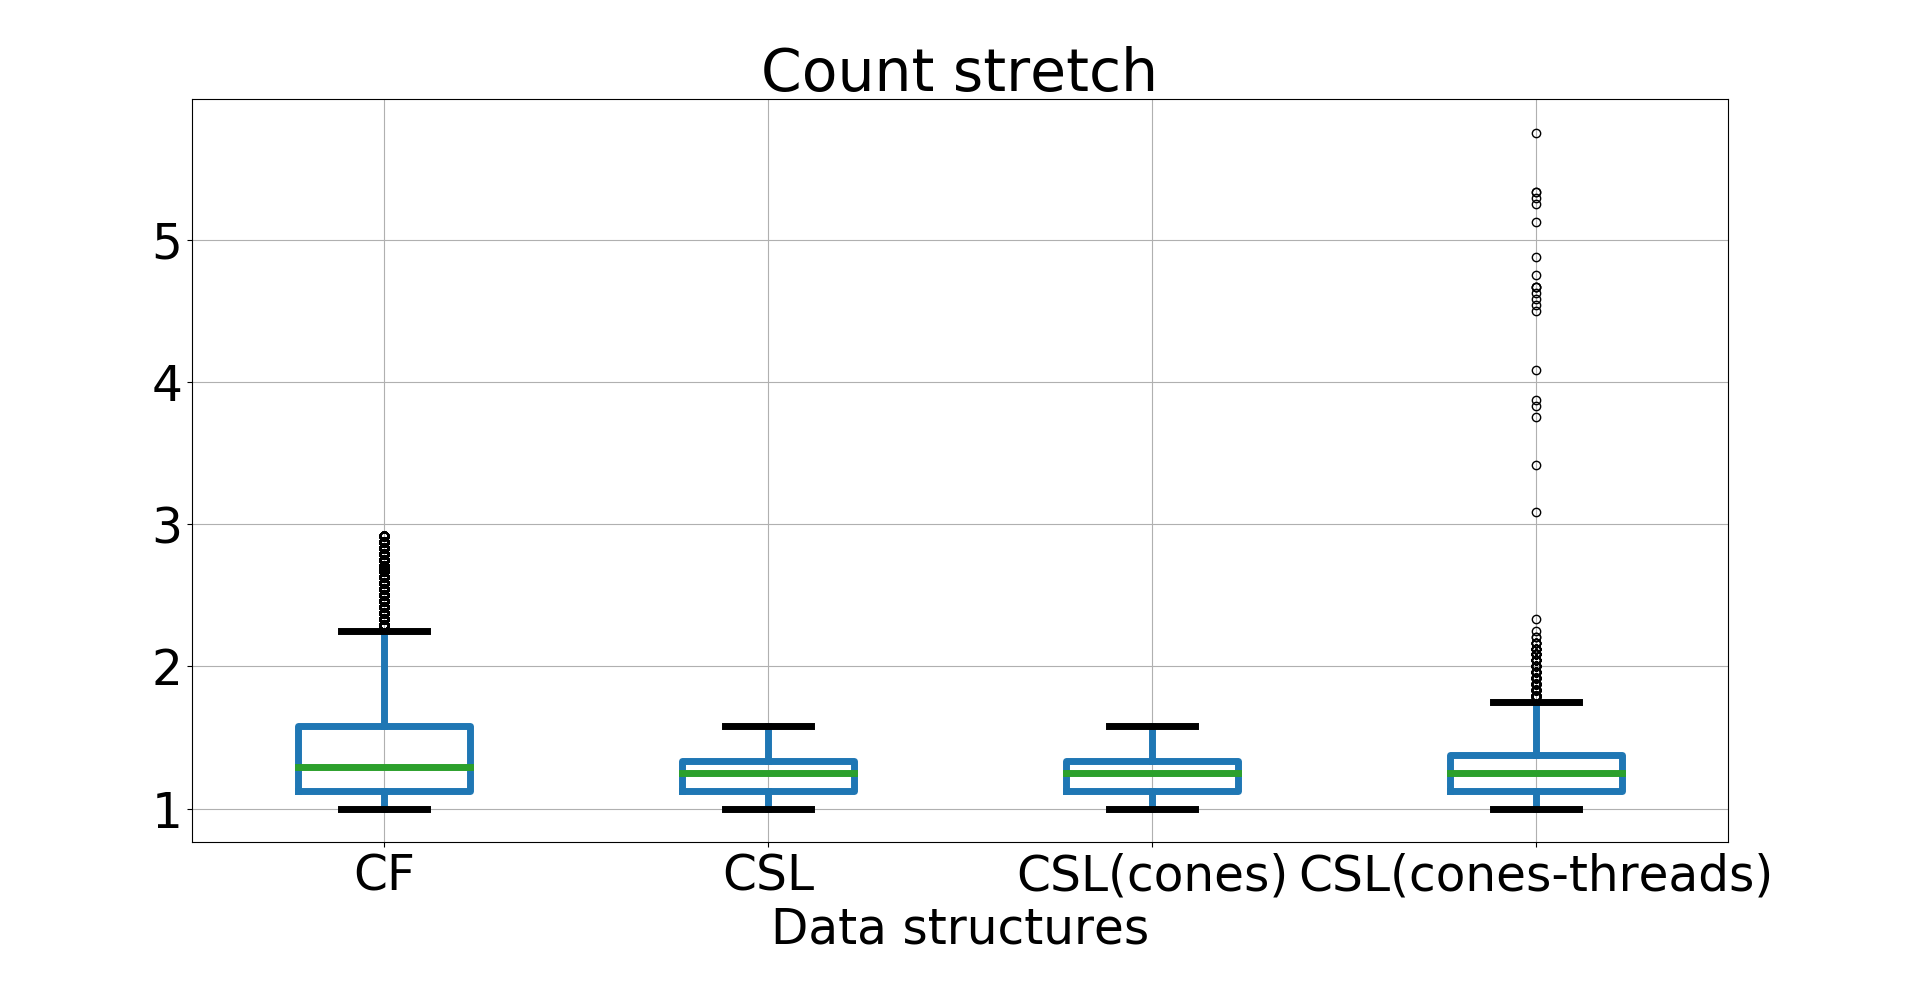
\includegraphics[width=\linewidth]{fig/countstretch-lifetime-r23-l4-g4-all_new_updated_fliers.png}
  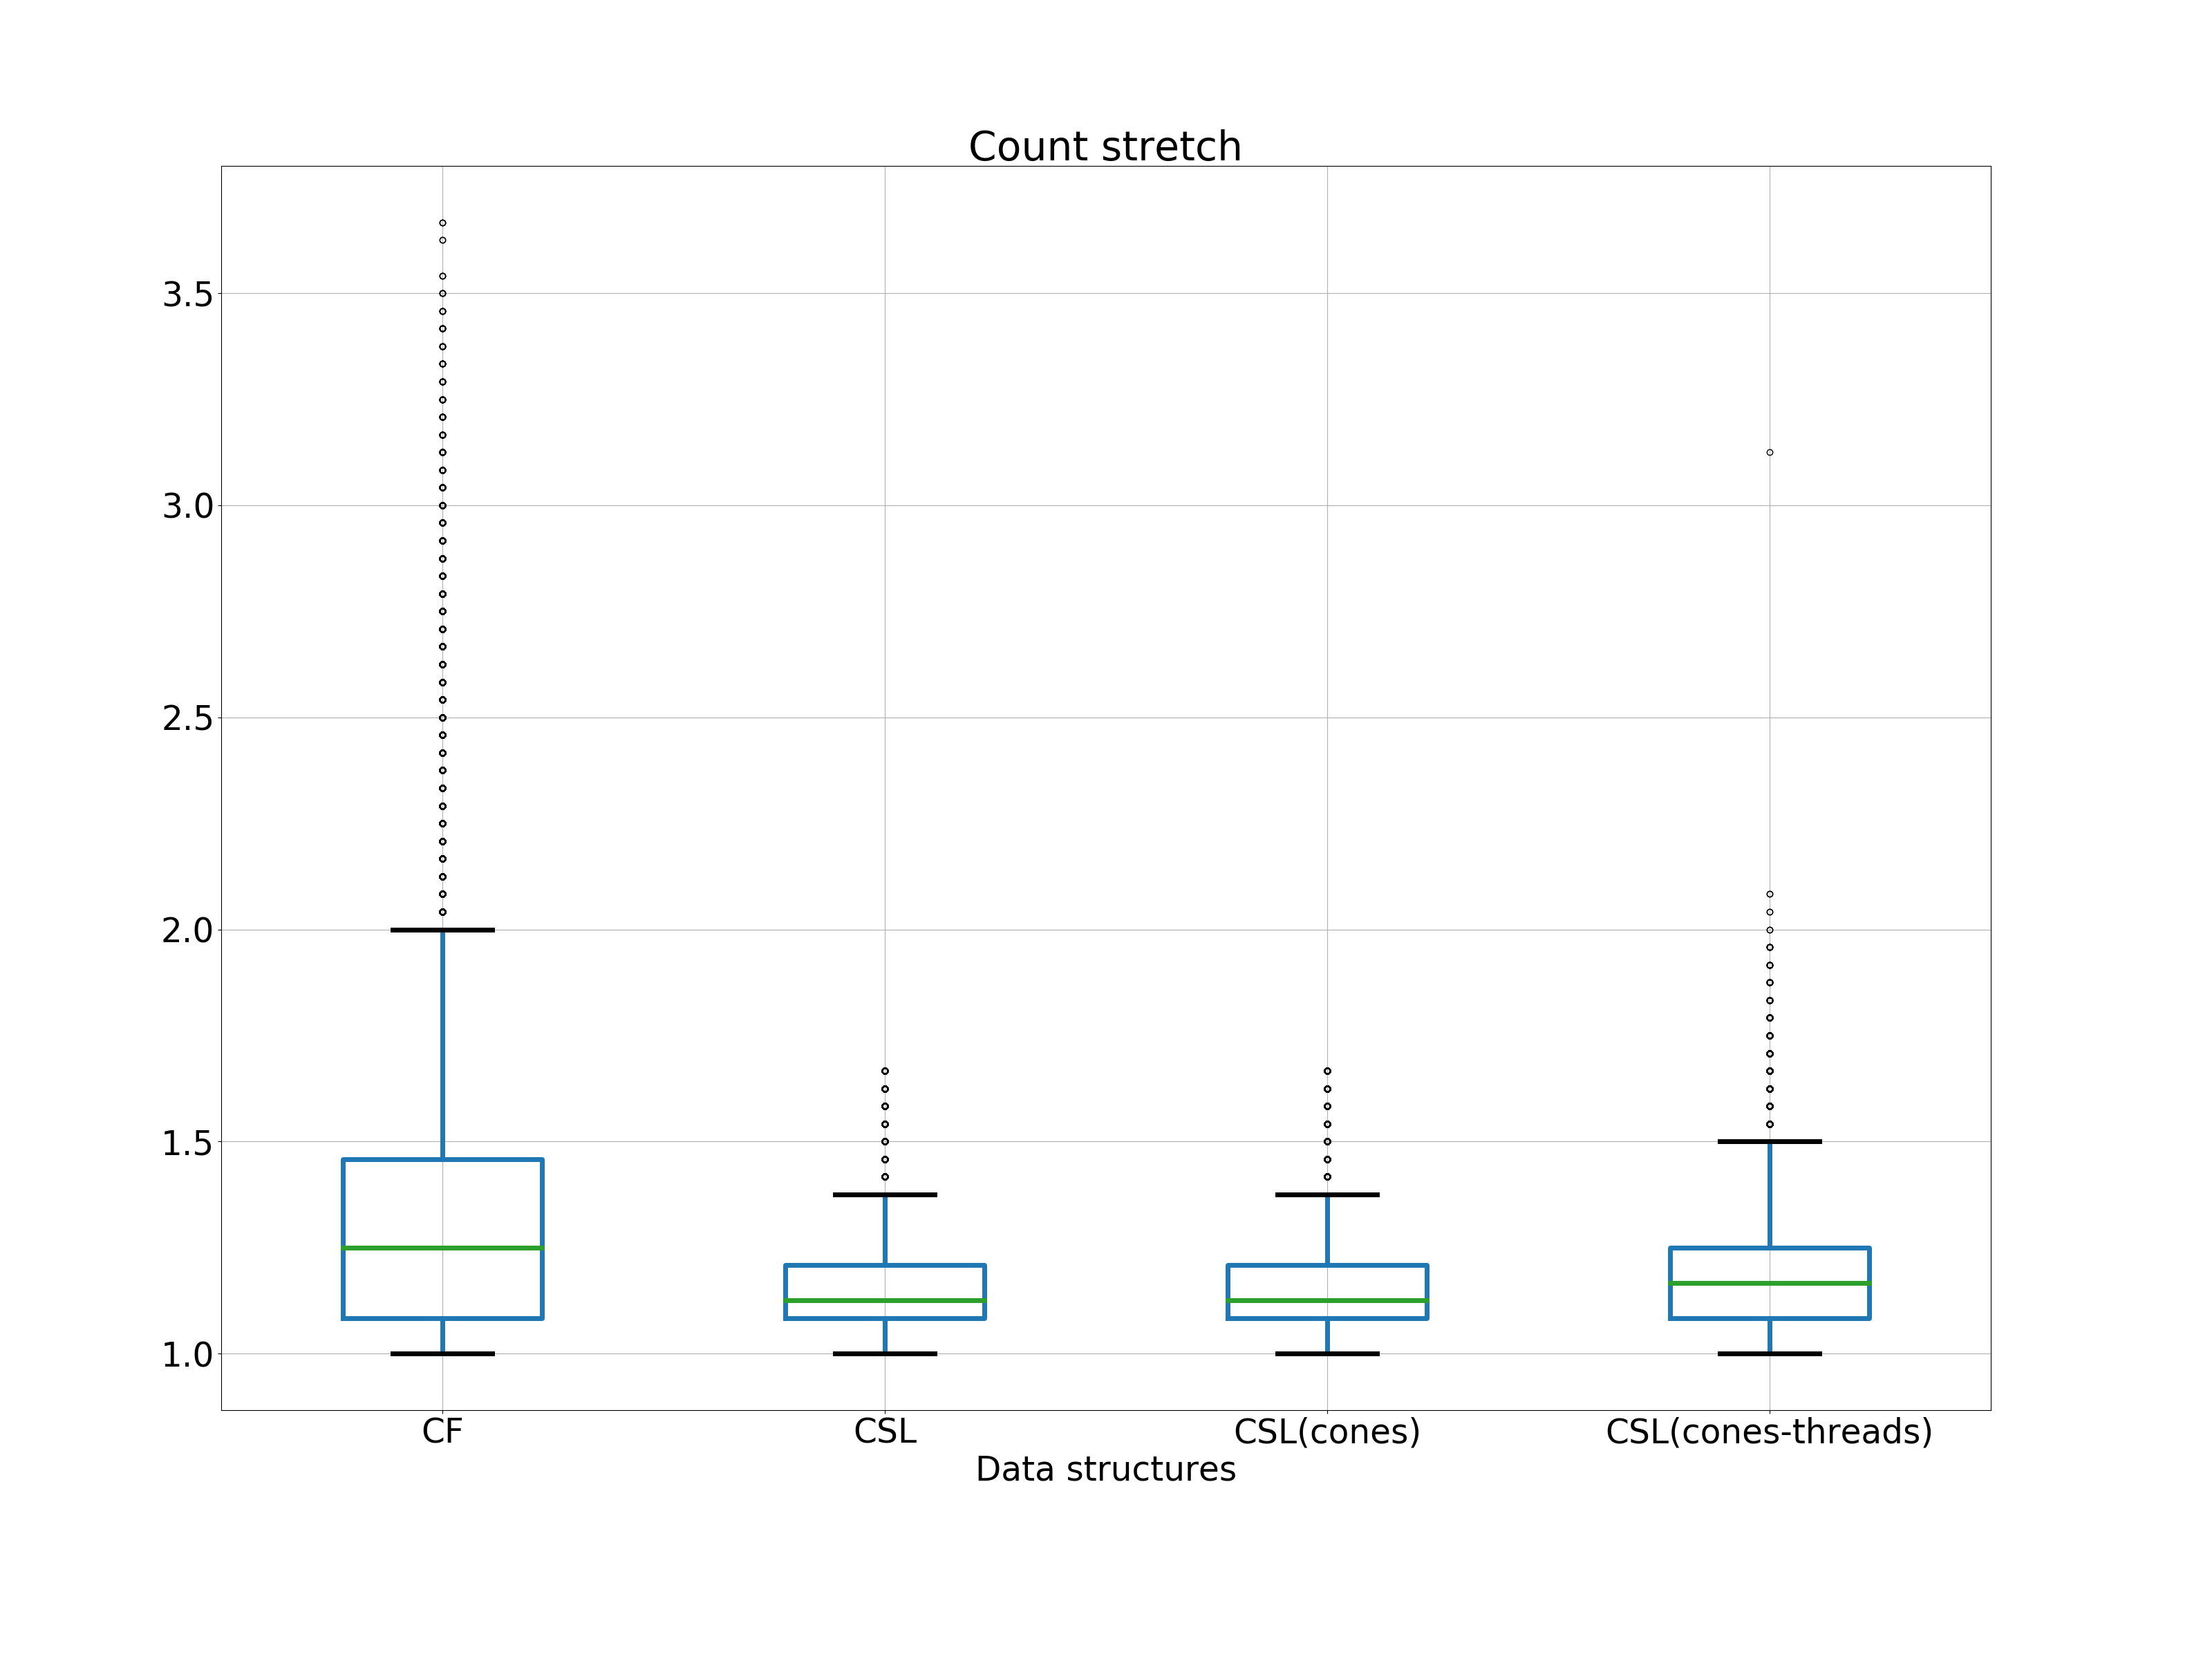
\includegraphics[width=\linewidth]{../LERT-src/sigmod20_figs/countstretch-dist.png}
  \captionsetup{margin=.5cm}
  \caption{Distribution of count stretch of different
  data structures.}
  \label{fig:countstretch}
\end{subfigure}
%
\begin{subfigure}{.33\textwidth}
  \centering
  %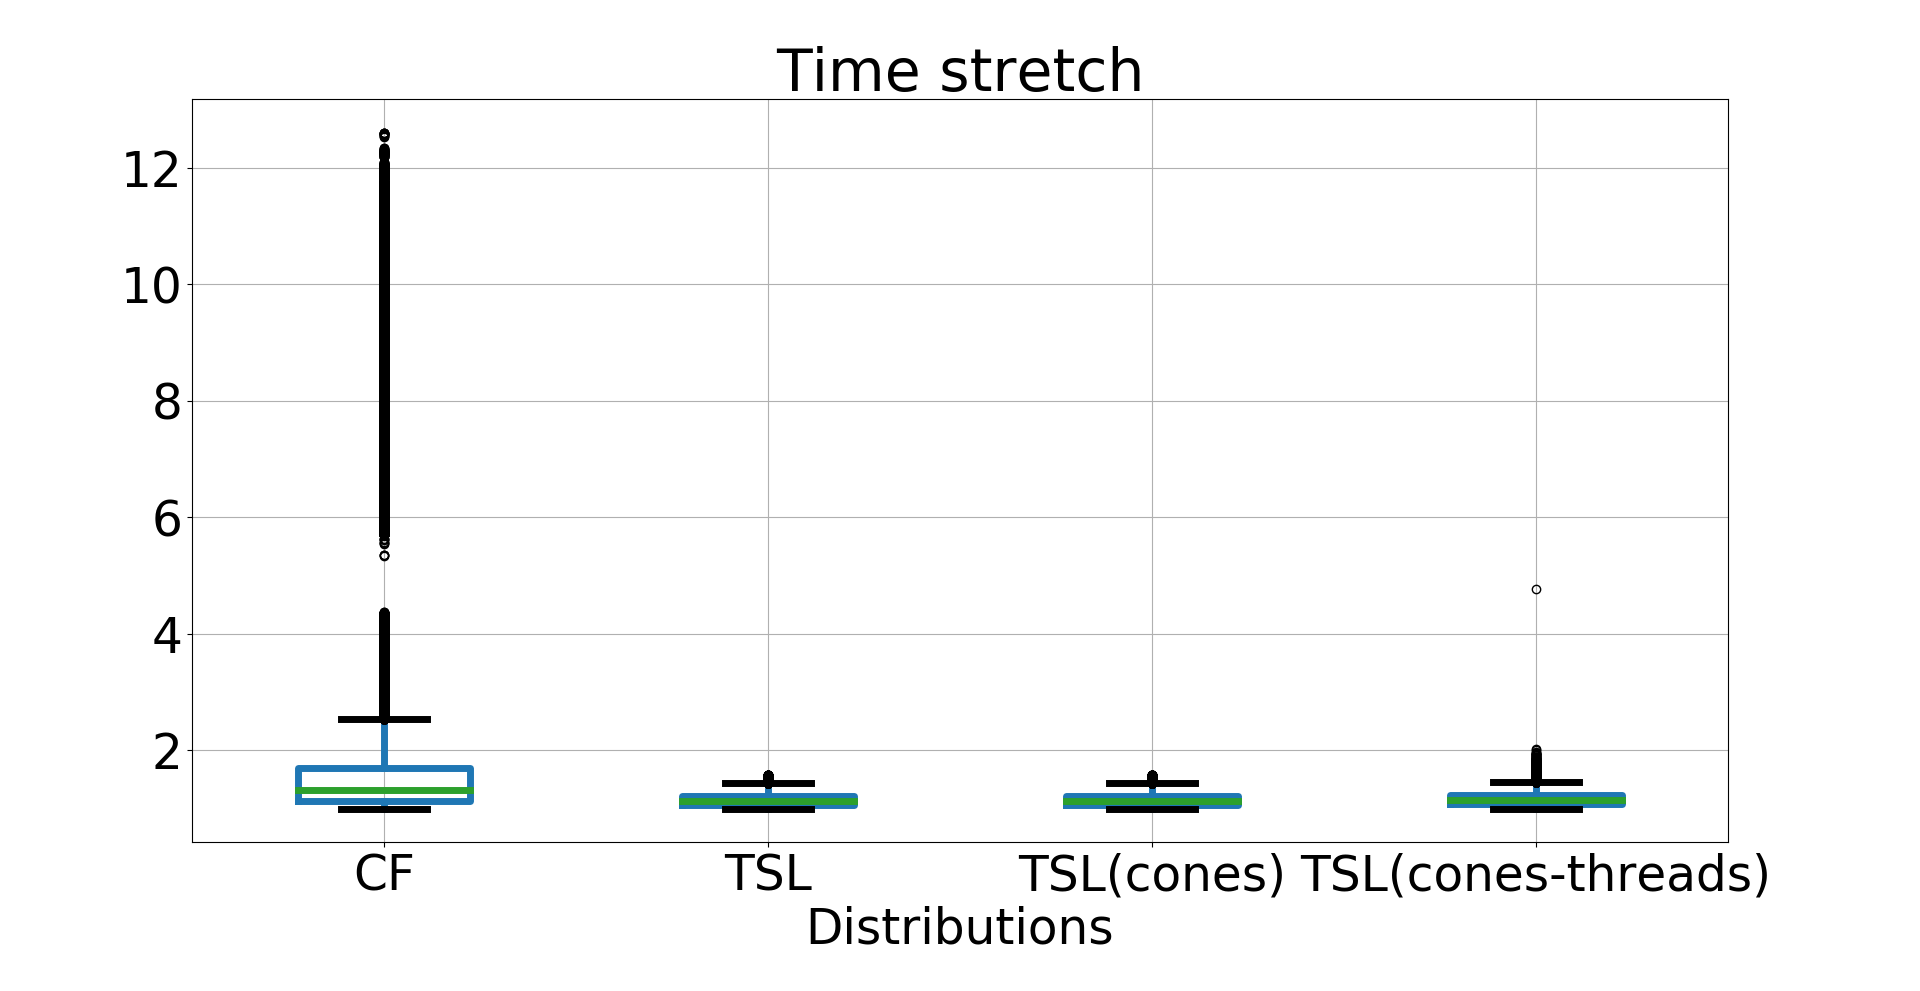
\includegraphics[width=\linewidth]{fig/timestretch-lifetime-r23-l4-g4-all_new_updated_fliers.png}
  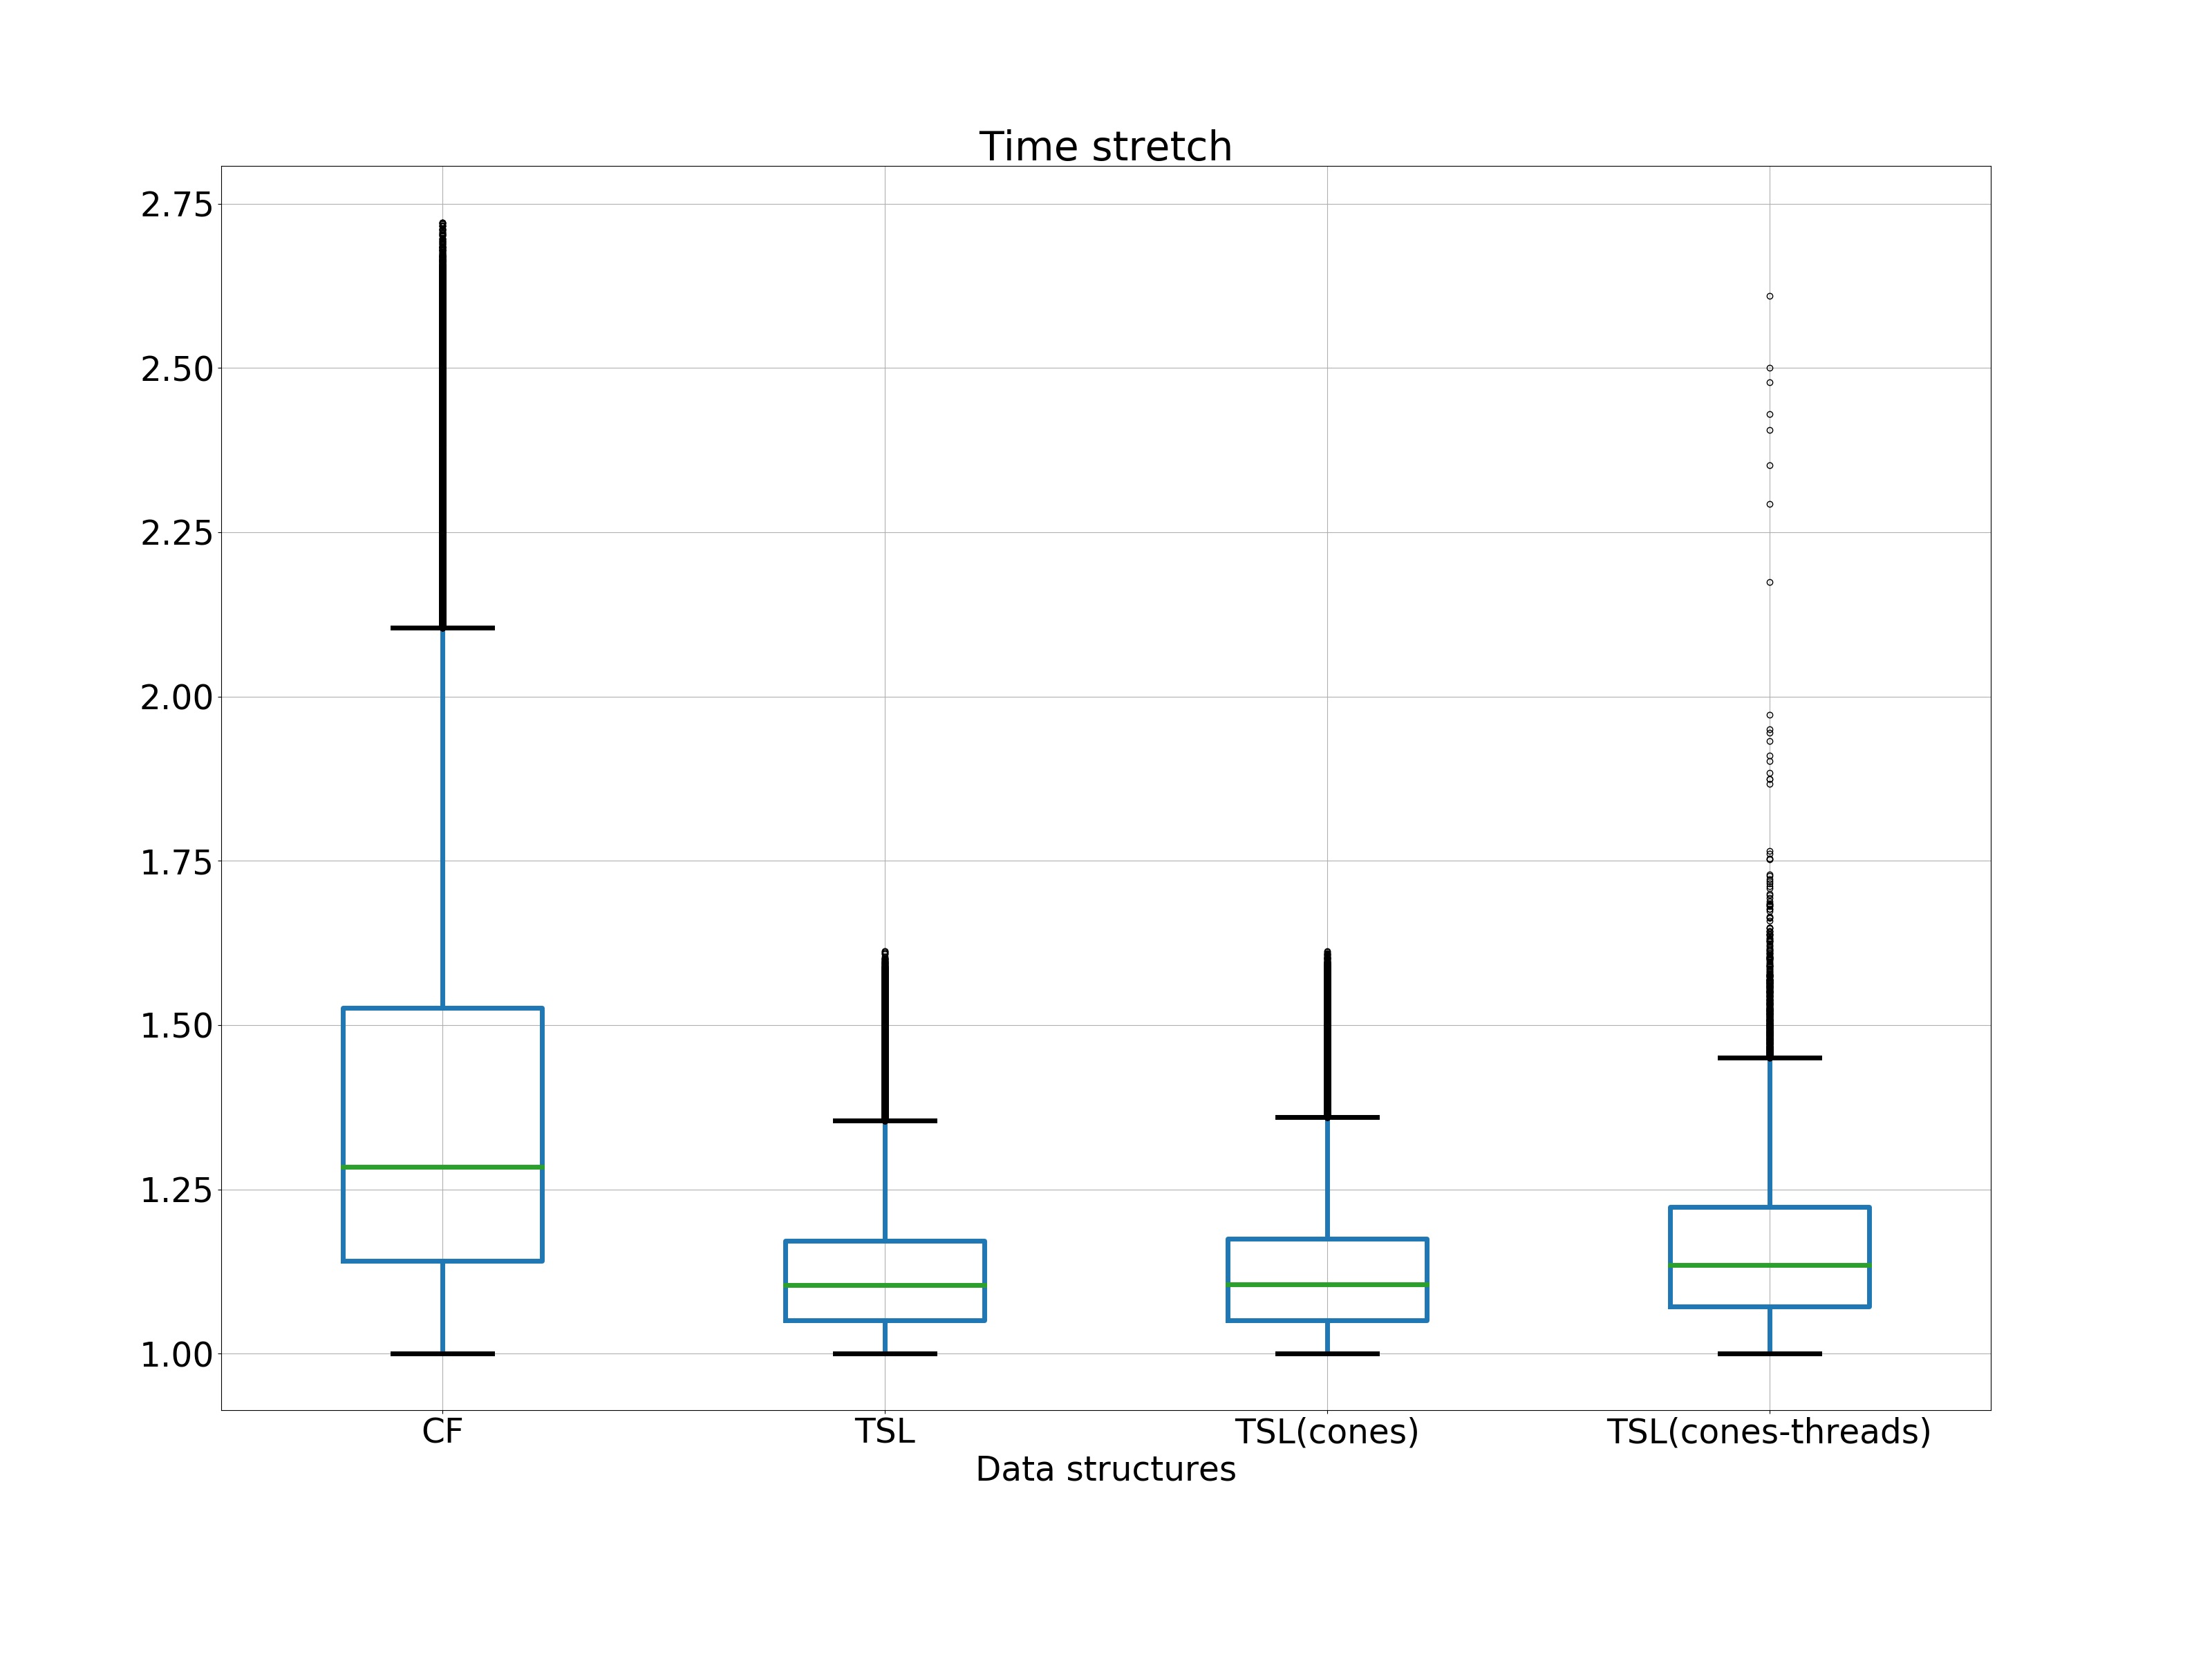
\includegraphics[width=\linewidth]{../LERT-src/sigmod20_figs/timestretch-dist.png}
  \captionsetup{margin=.5cm}
  \caption{Distribution of time stretch of different
  data structures.}
  \label{fig:timestretch}
\end{subfigure}
%
\begin{subfigure}{.33\textwidth}
  \centering
  %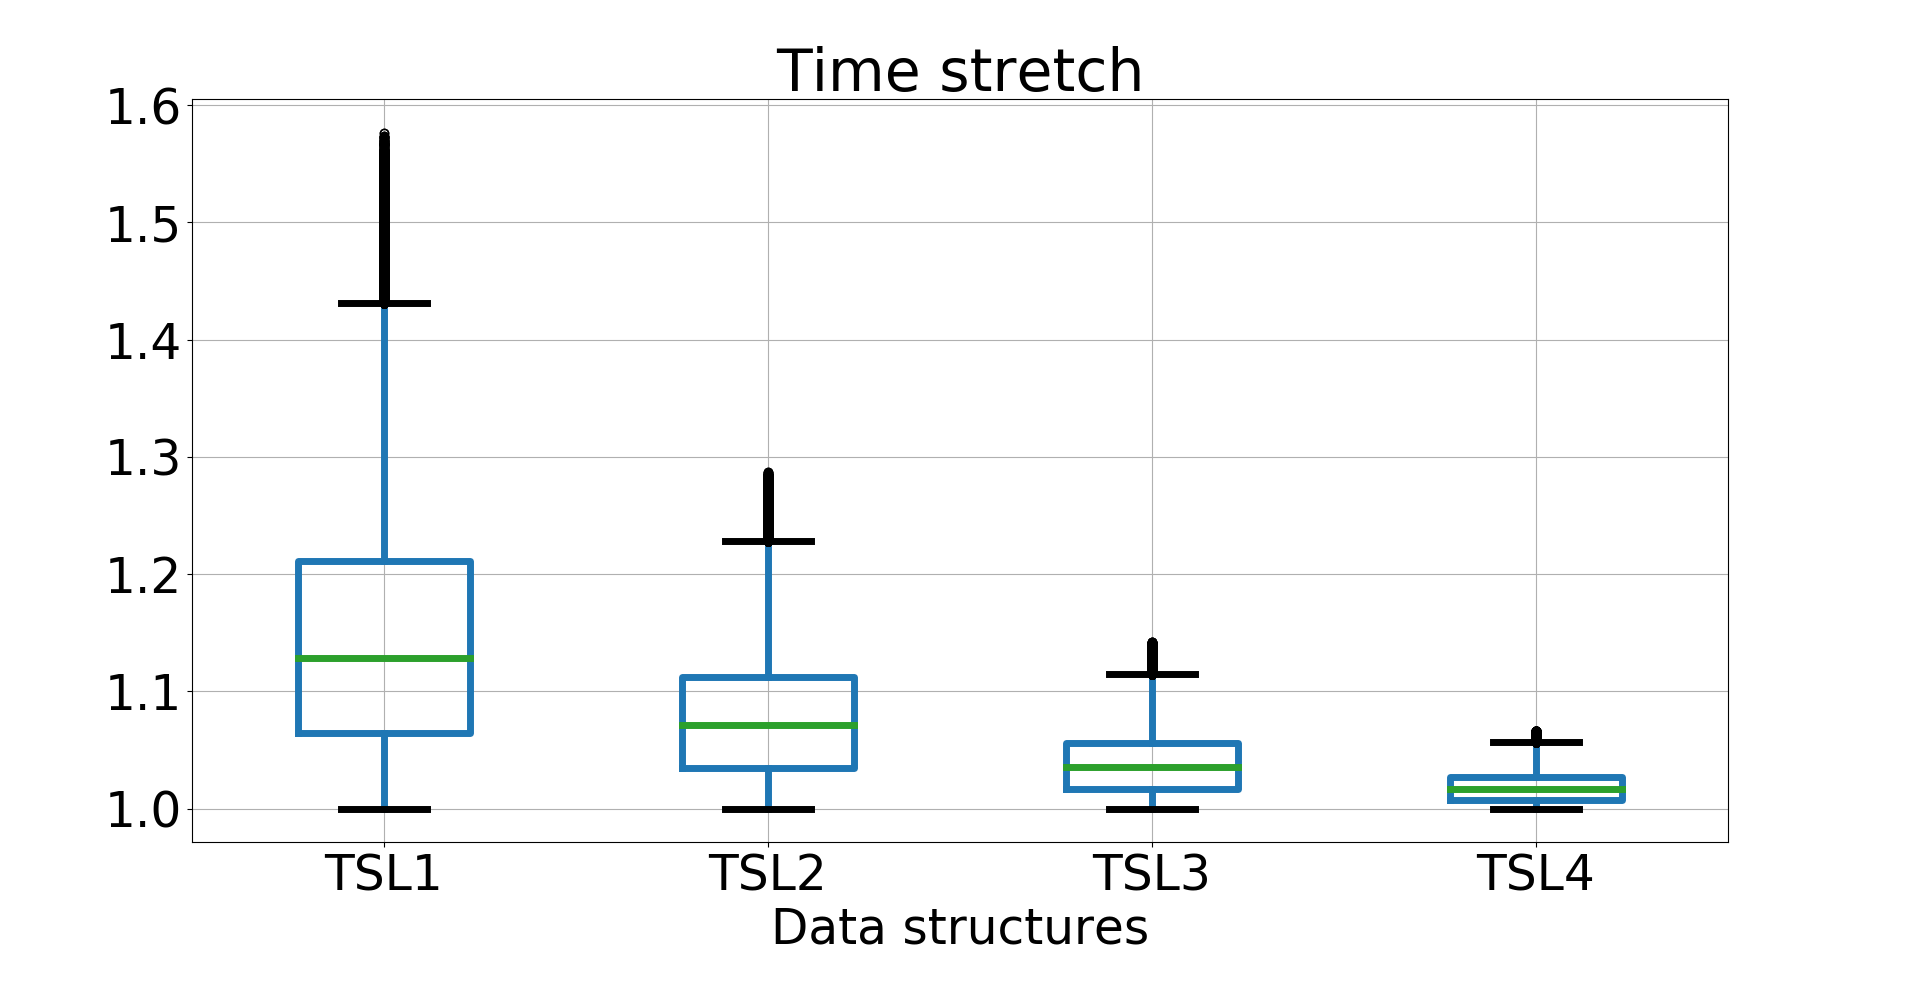
\includegraphics[width=\linewidth]{fig/timestretch-lifetime-r23-l4-g4-a1to4_new_fliers.png}
  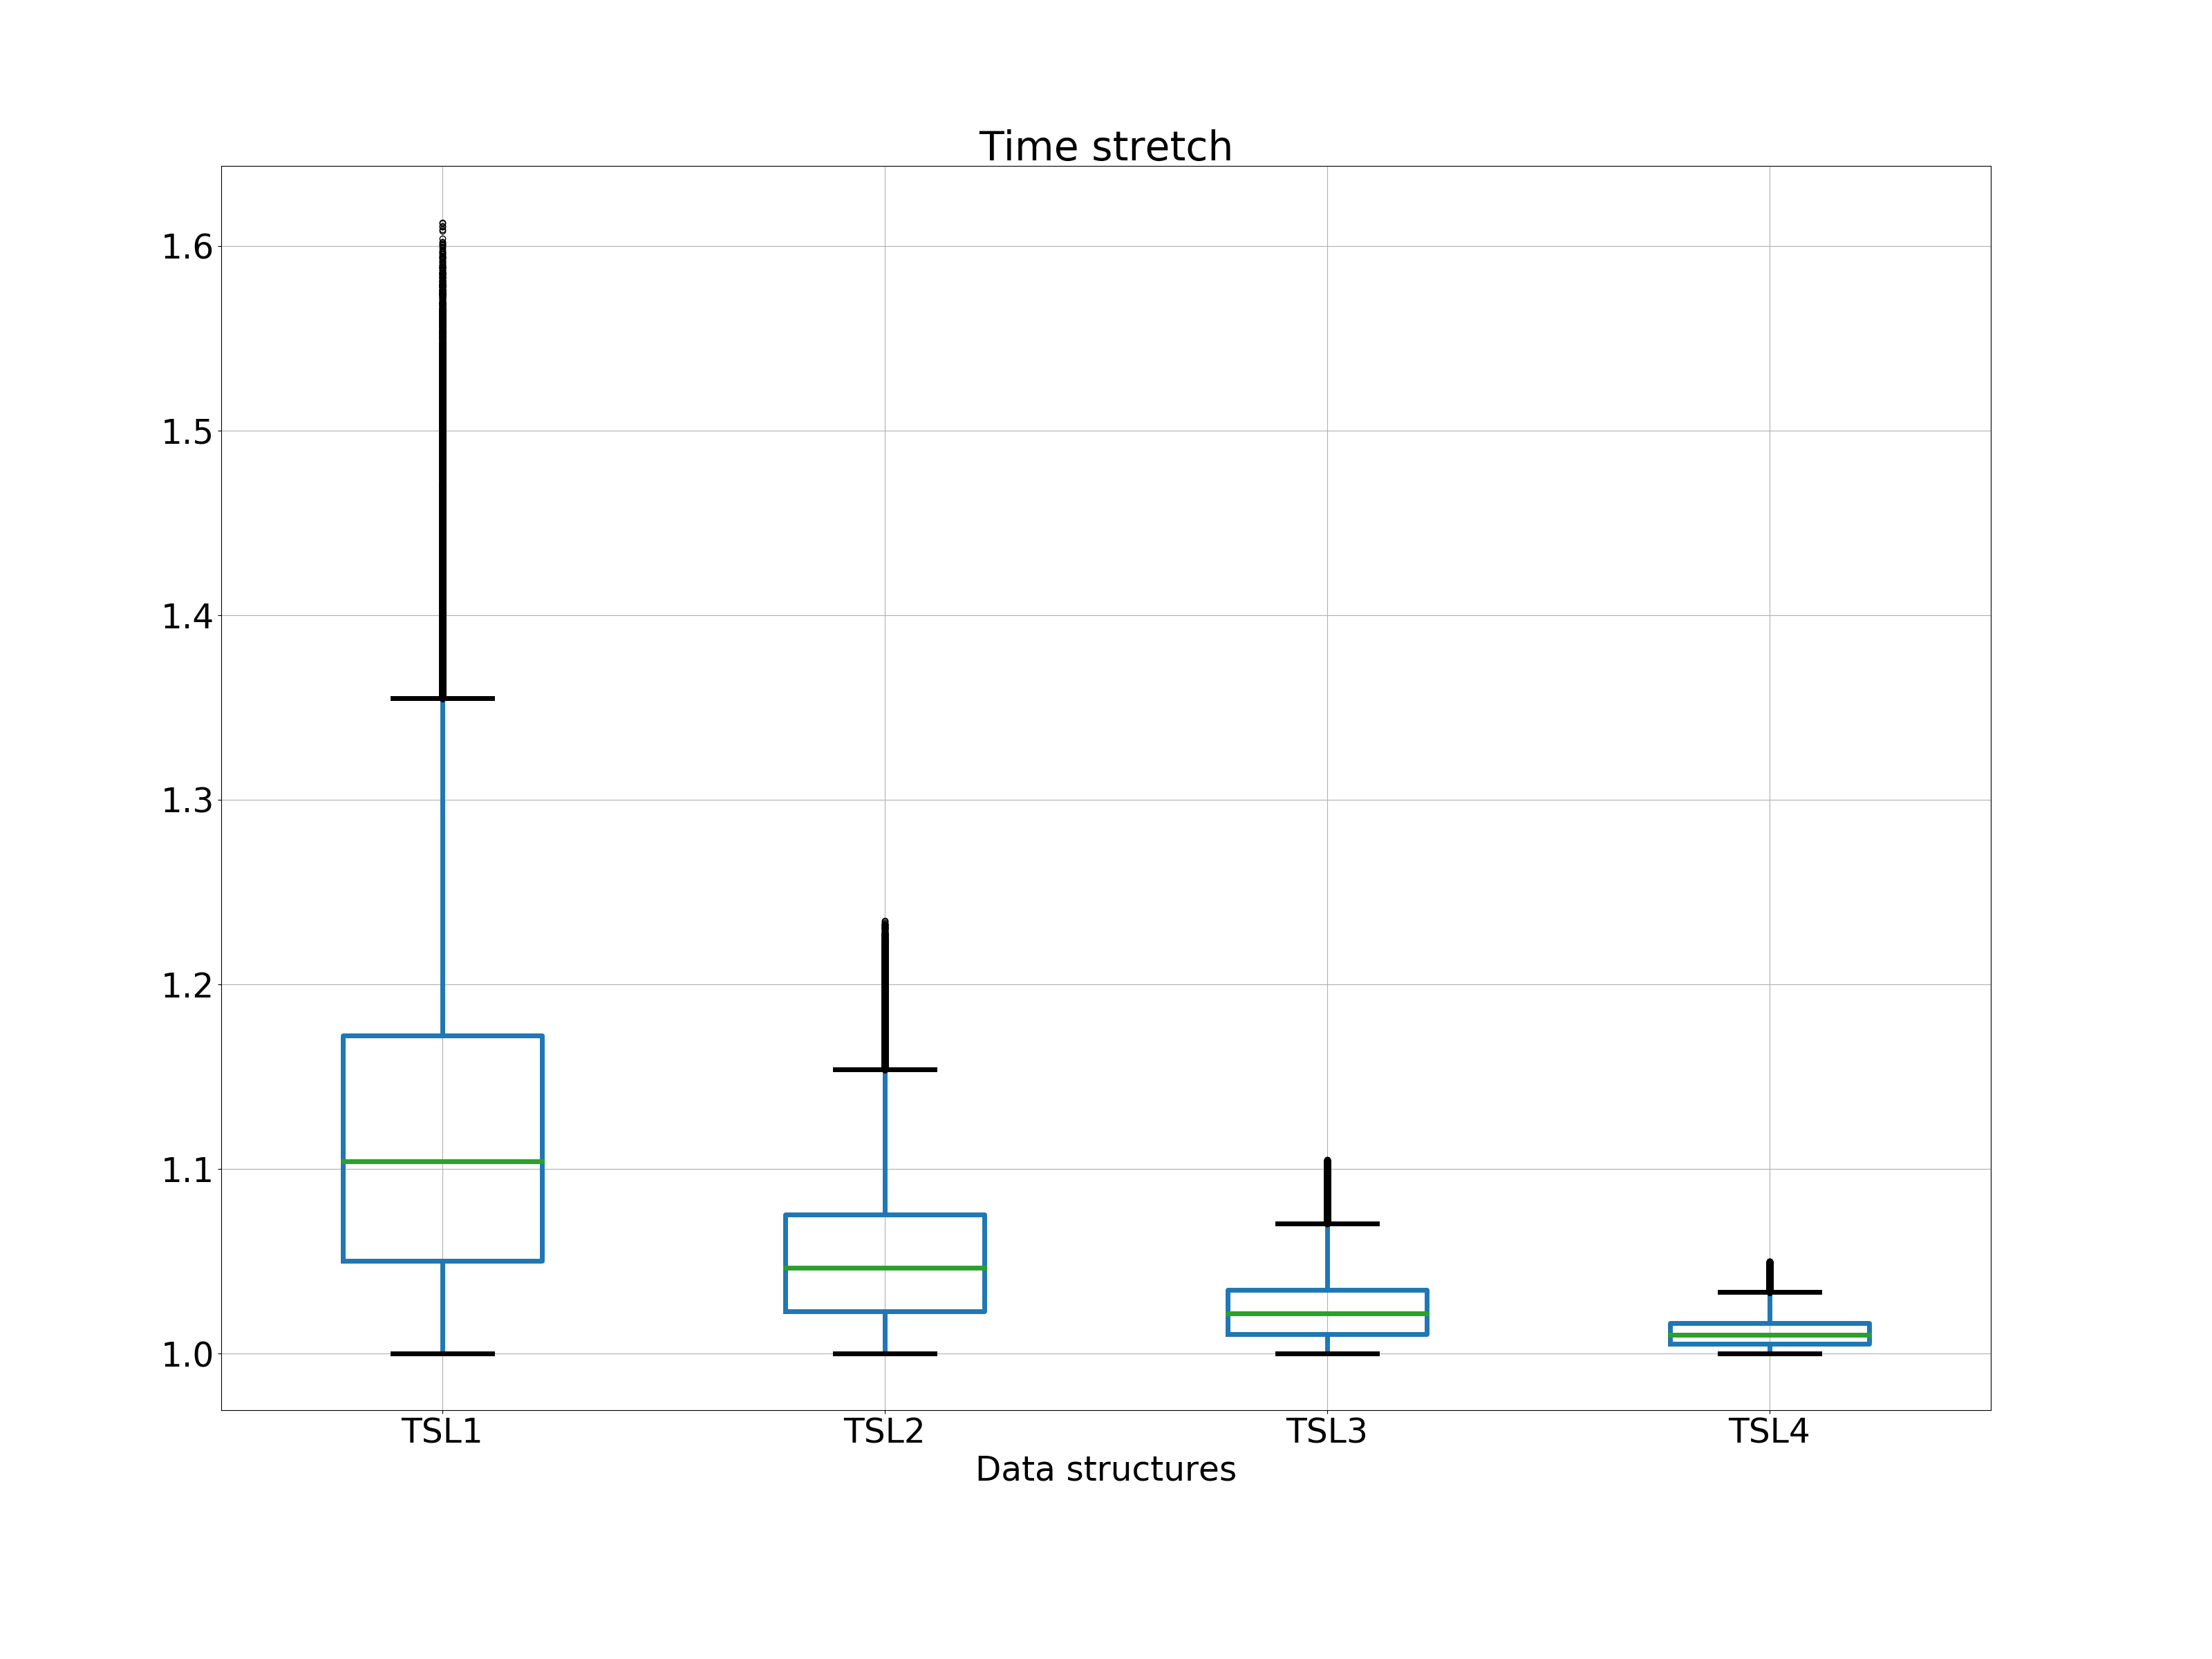
\includegraphics[width=\linewidth]{../LERT-src/sigmod20_figs/timestretch-a-dist.png}
  \captionsetup{margin=.5cm}
  \caption{Distribution of time stretch in the \ts for
  different \boldmath  $\alpha$ values.}
  \label{fig:timeliness-timestretch}
\end{subfigure}
%
}
\caption{\boldmath Data structure configuration: RAM level: 8388608 slots in
    the CQF, levels: 4, growth factor: 4, level thresholds: (2, 4, 8), cones: 8, threads: 8, number of
  observations: 512M.
%
  Data structures: Cascade filter (CF), \cs (CSL),
  \ts (TSL), (CSL and TSL) with cones, (CSL and TSL) with cones and threads.
  \Ts with age bits 1 (TSL1) $\alpha=1$, 2 (TSL2) $\alpha=0.33$, 3 (TSL3)
  $\alpha=0.14$, and 4 (TSL4) $\alpha=0.06$.
} 
\label{fig:timeliness}
\end{figure*}

\begin{figure}
{\centering
\begin{subfigure}{.50\textwidth}
  \centering
  %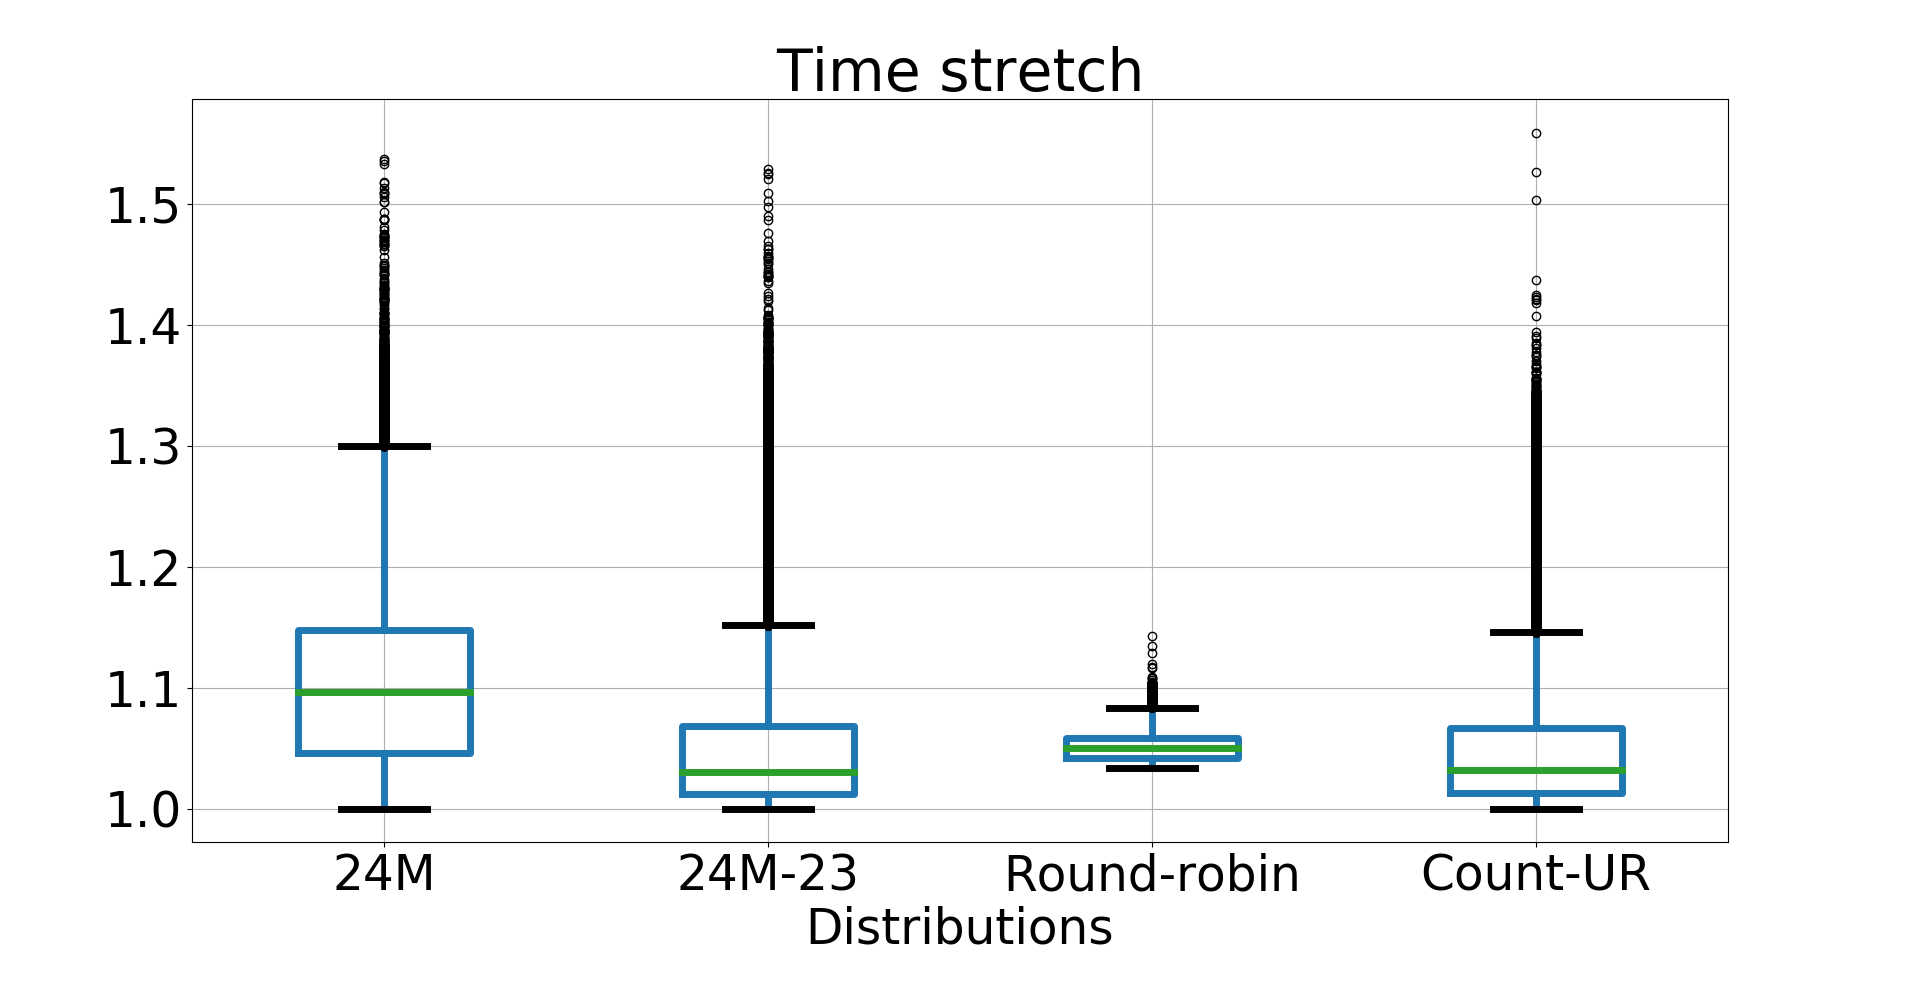
\includegraphics[width=.8\linewidth]{fig/timestretch-lifetime-r23-l4-g4-a1-arb-all_fliers.png}
  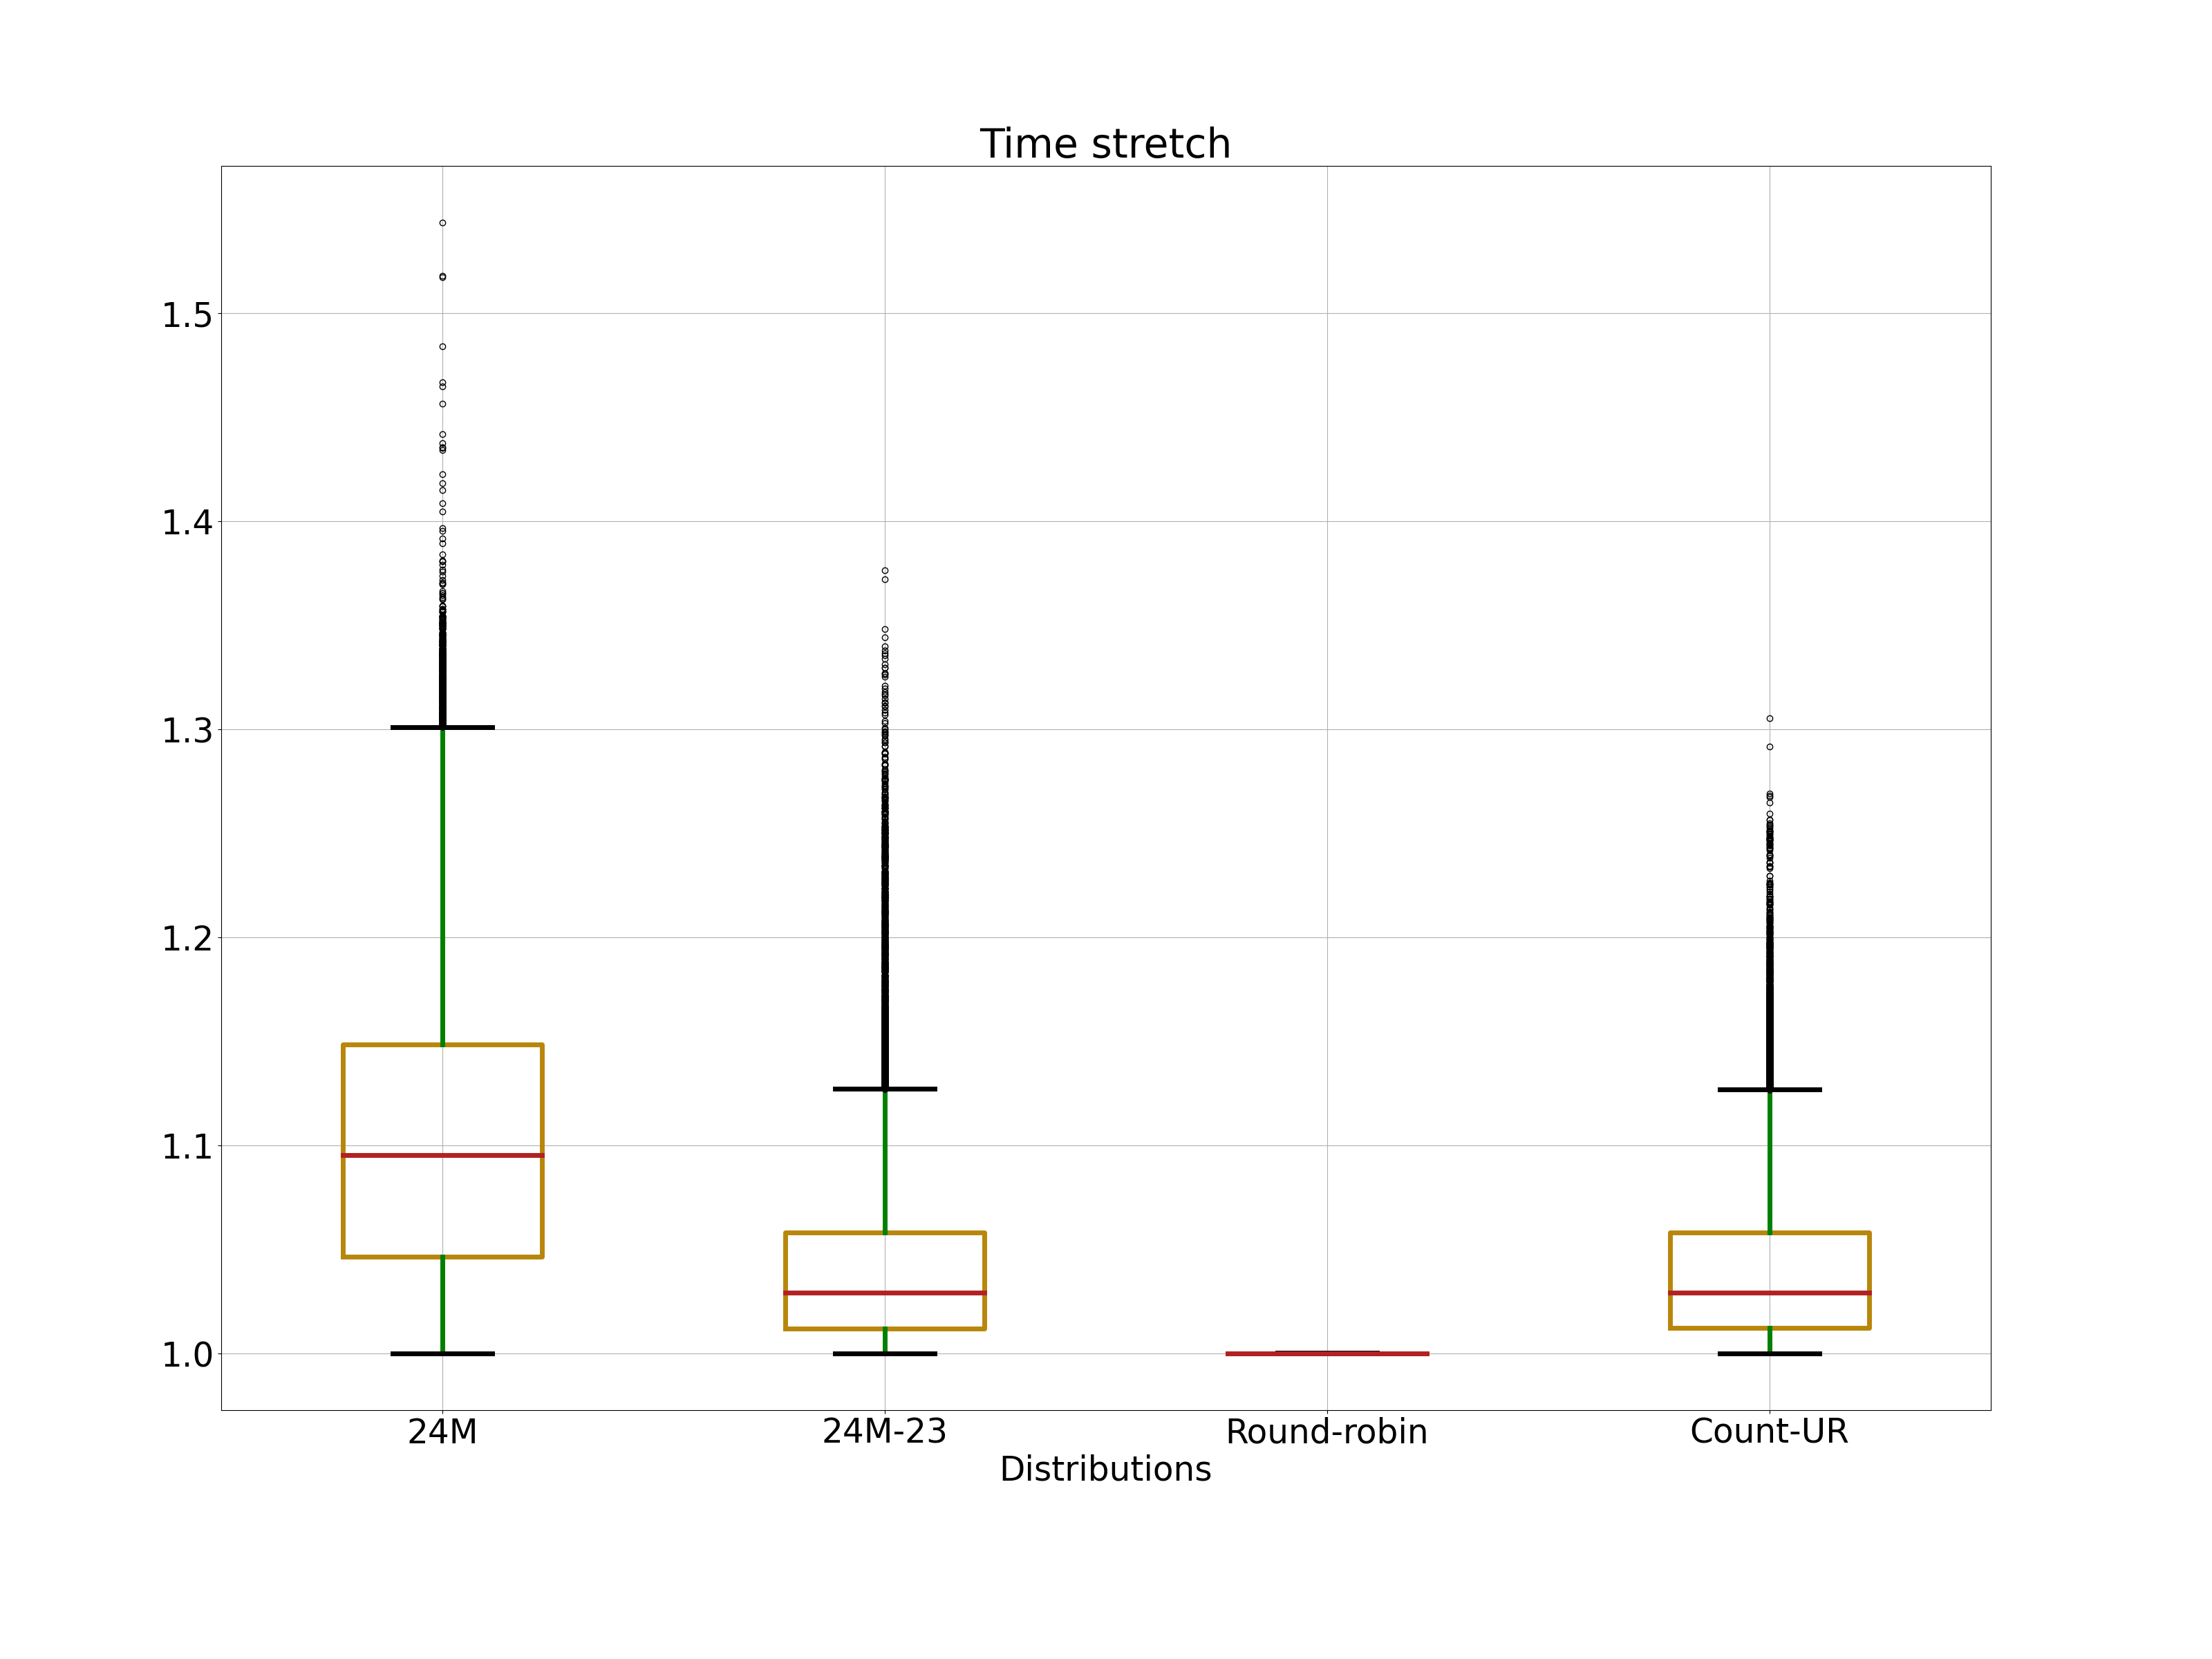
\includegraphics[width=\linewidth]{../LERT-src/sigmod20_figs/timestretch-arb-dist.png}
  \captionsetup{margin=.5cm}
  \caption{Distribution of time stretch for different
    distributions. These distributions are described in~\Cref{diff_dist}.}
  \label{fig:timestretch-arb}
\end{subfigure}
\\
\begin{subfigure}{.50\textwidth}
  \centering
  %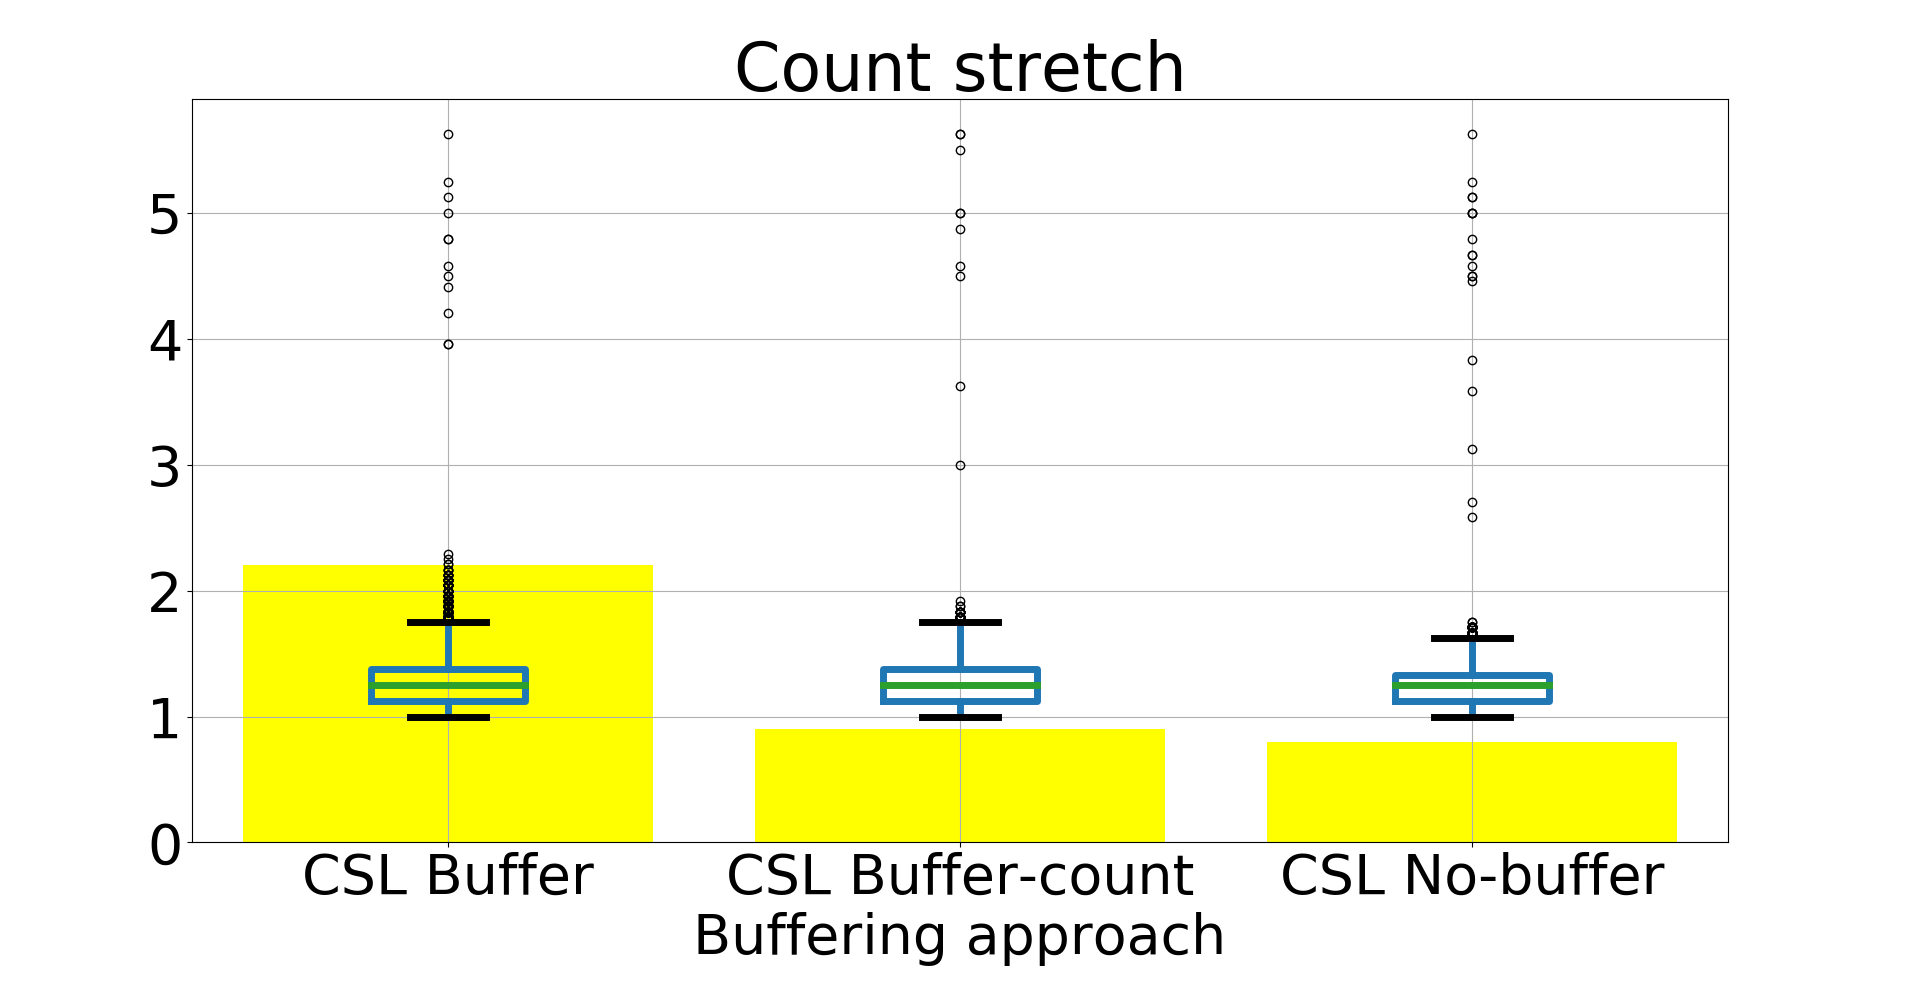
\includegraphics[width=.8\linewidth]{fig/countstretch-lifetime-r23-l4-g4-c8-t8-buffering-overlay-new-fliers.png}
  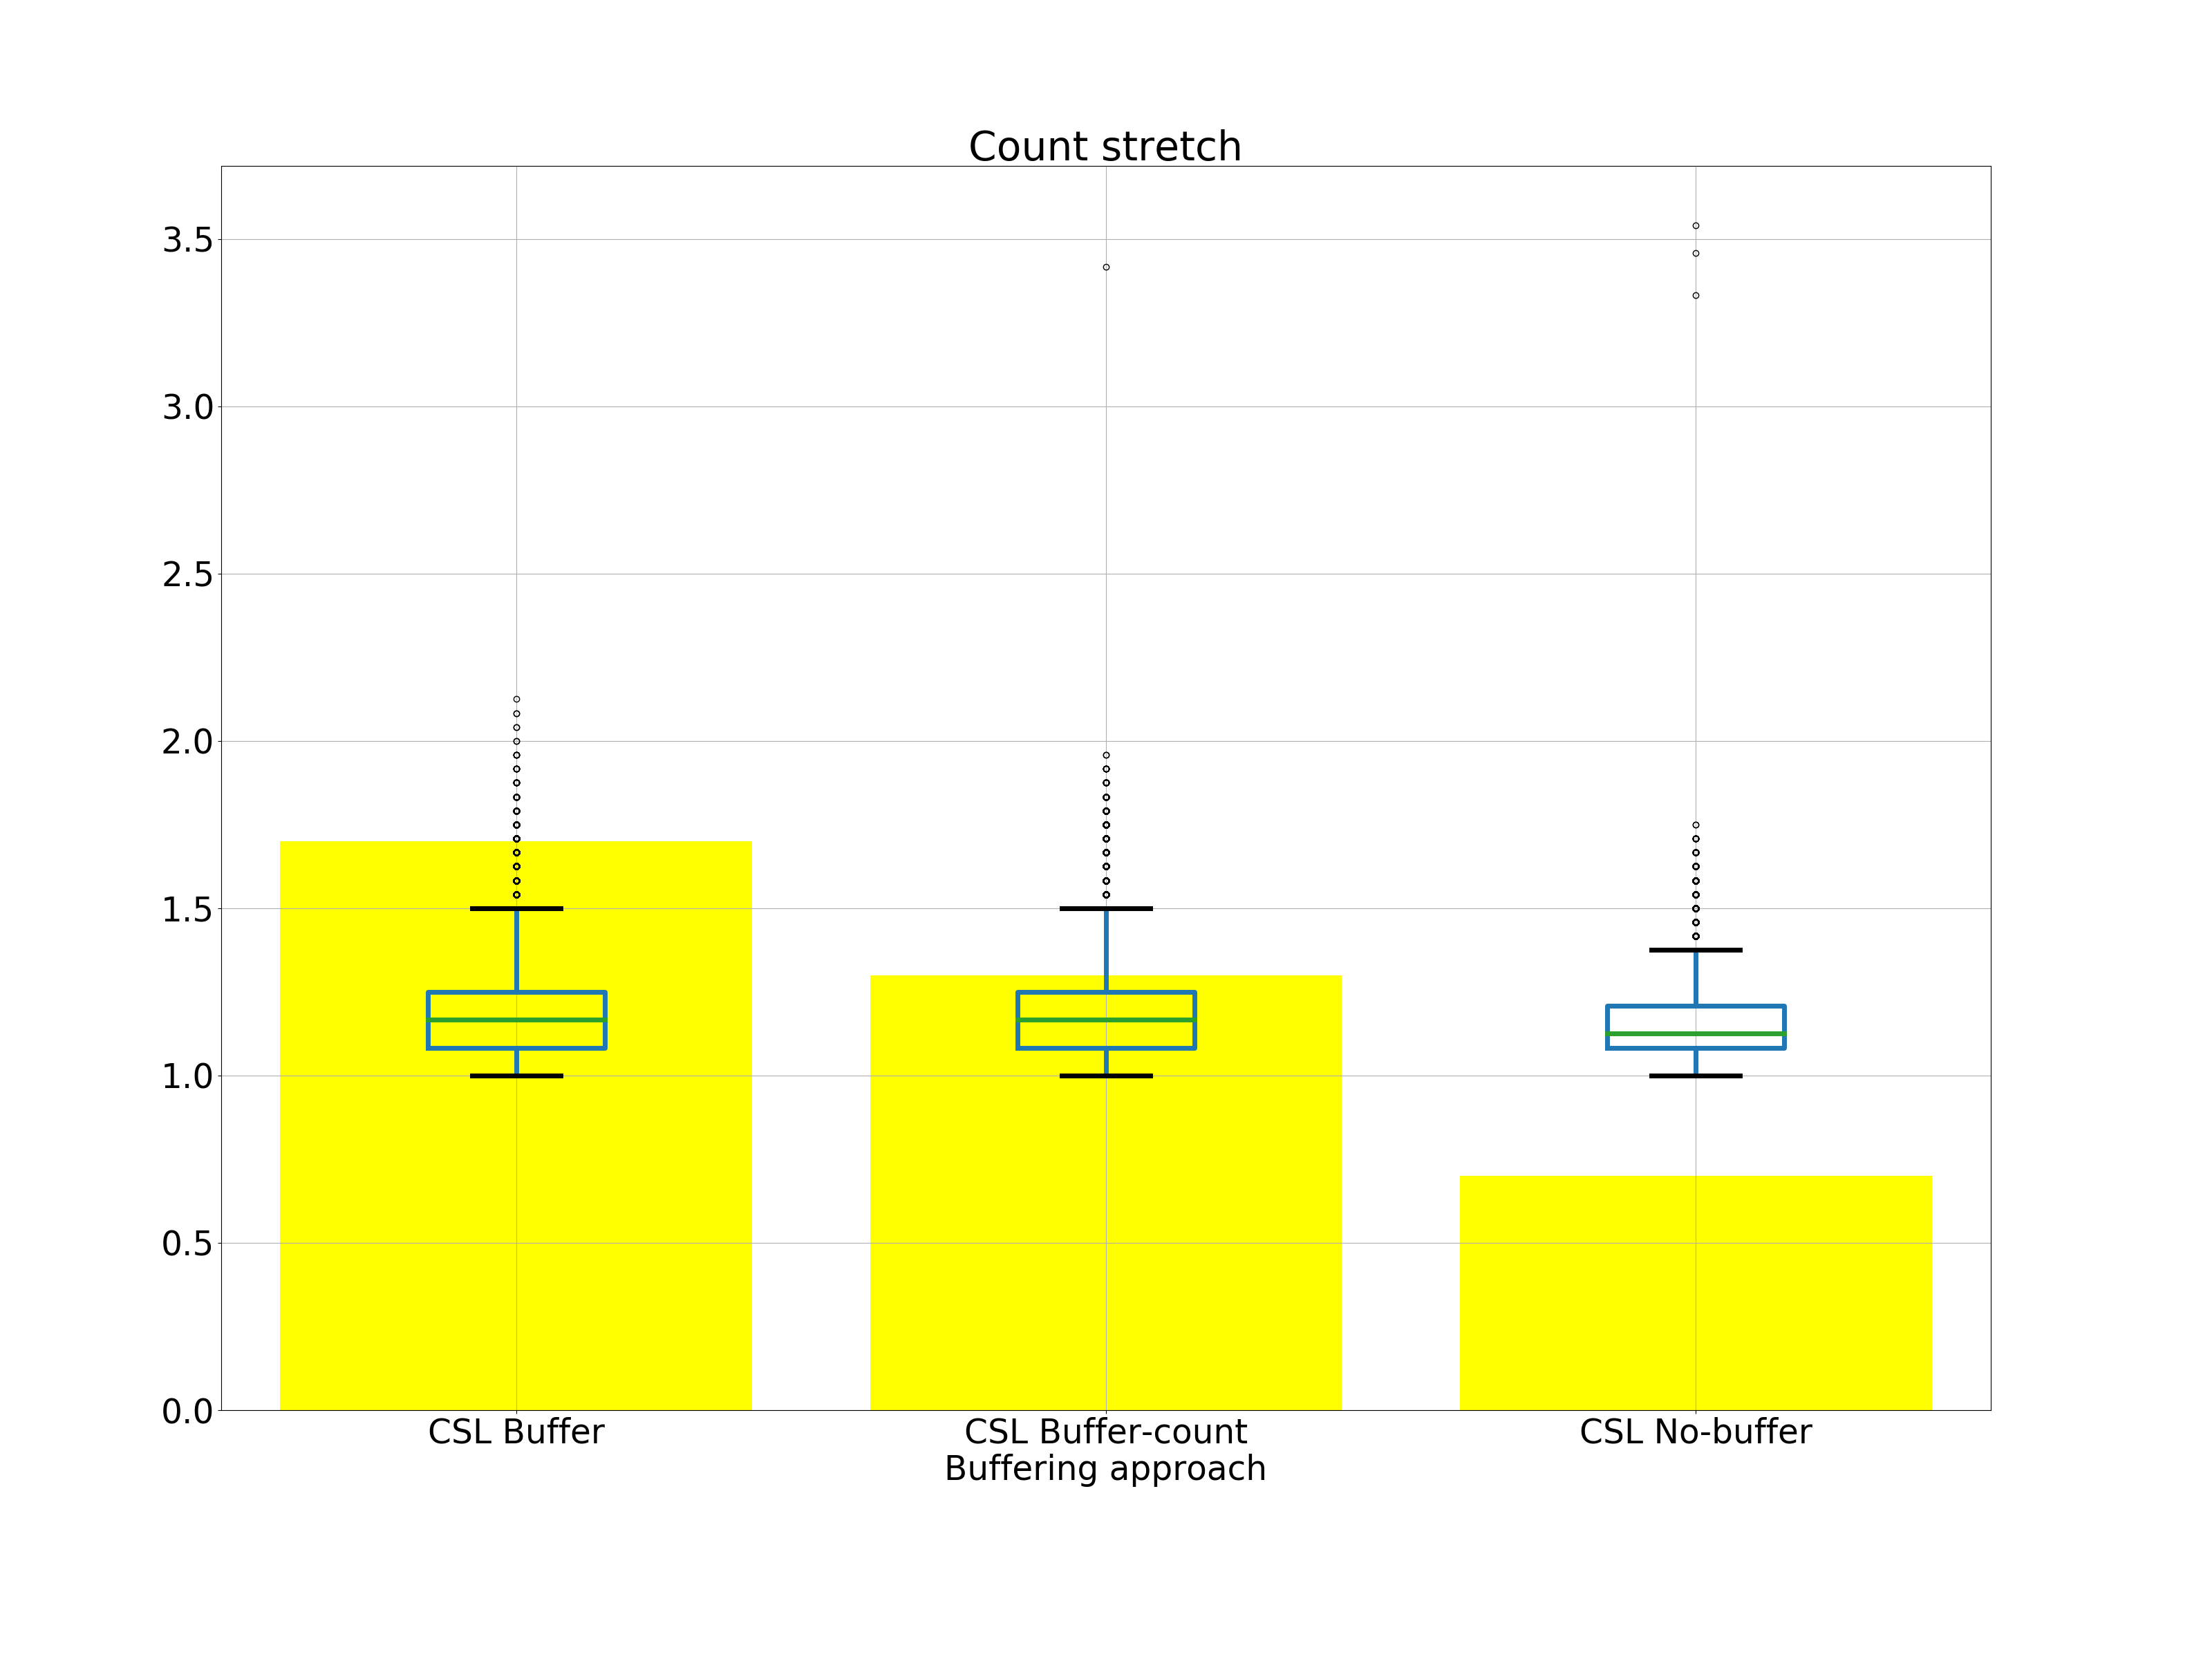
\includegraphics[width=\linewidth]{../LERT-src/sigmod20_figs/countstretch-buffer-dist.png}
  \captionsetup{margin=.5cm}
  \caption{Distribution of count stretch with different
  buffering strategies. Bars show the average insertion throughput
  (Million insertions/sec) for each buffering strategy. Average insertion throughput when
  no-buffer is used is $2.7\times$ lower compared to when buffers are used.}
  \label{fig:countstretch-buffering}
\end{subfigure}
}
\caption{Data structure configuration: RAM level: 8388608 slots in
    the CQF, levels: 4, growth factor: 4, level thresholds for on-disk
    level: (2, 4, 8), cones: 8, threads: 8, number of
  observations: 512M.
}
\label{fig:roboustness}
\end{figure}


\begin{figure}
{\centering
\begin{subfigure}{.50\textwidth}
  \centering
  %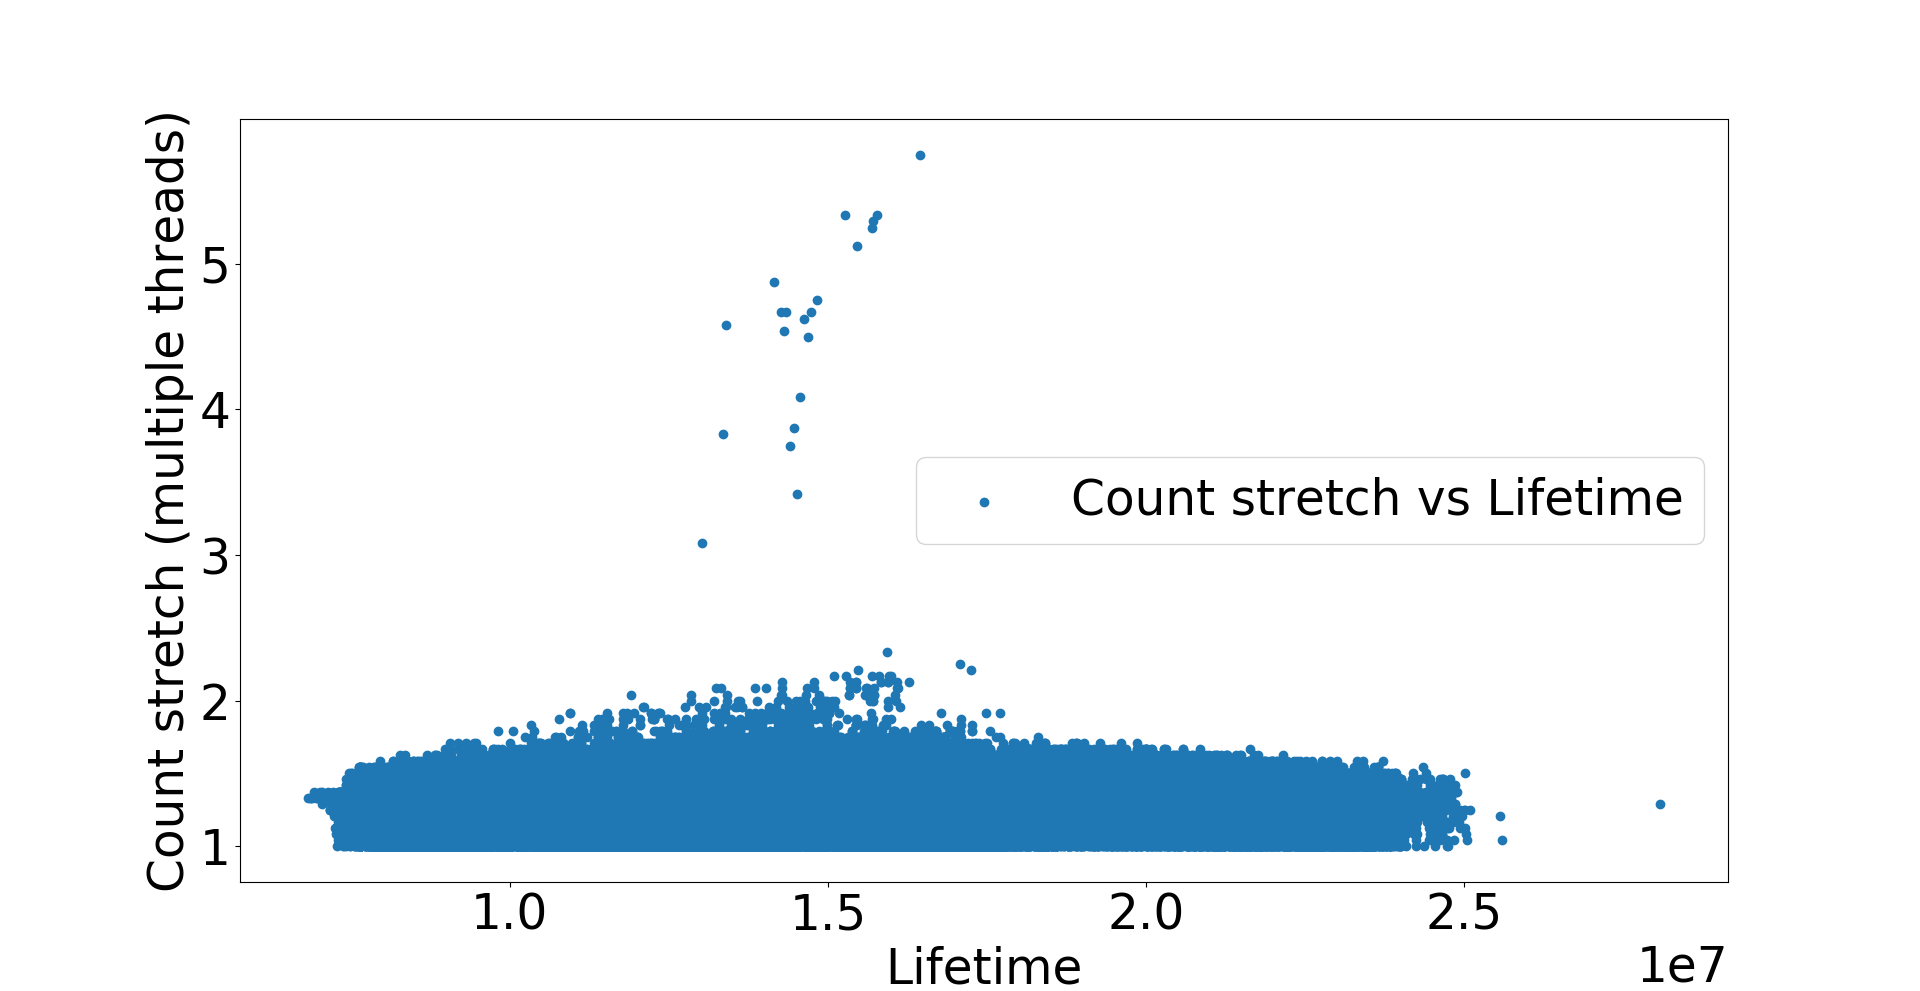
\includegraphics[width=.8\linewidth]{fig/Count-Stretch-Lifetime_r23_l4.png}
  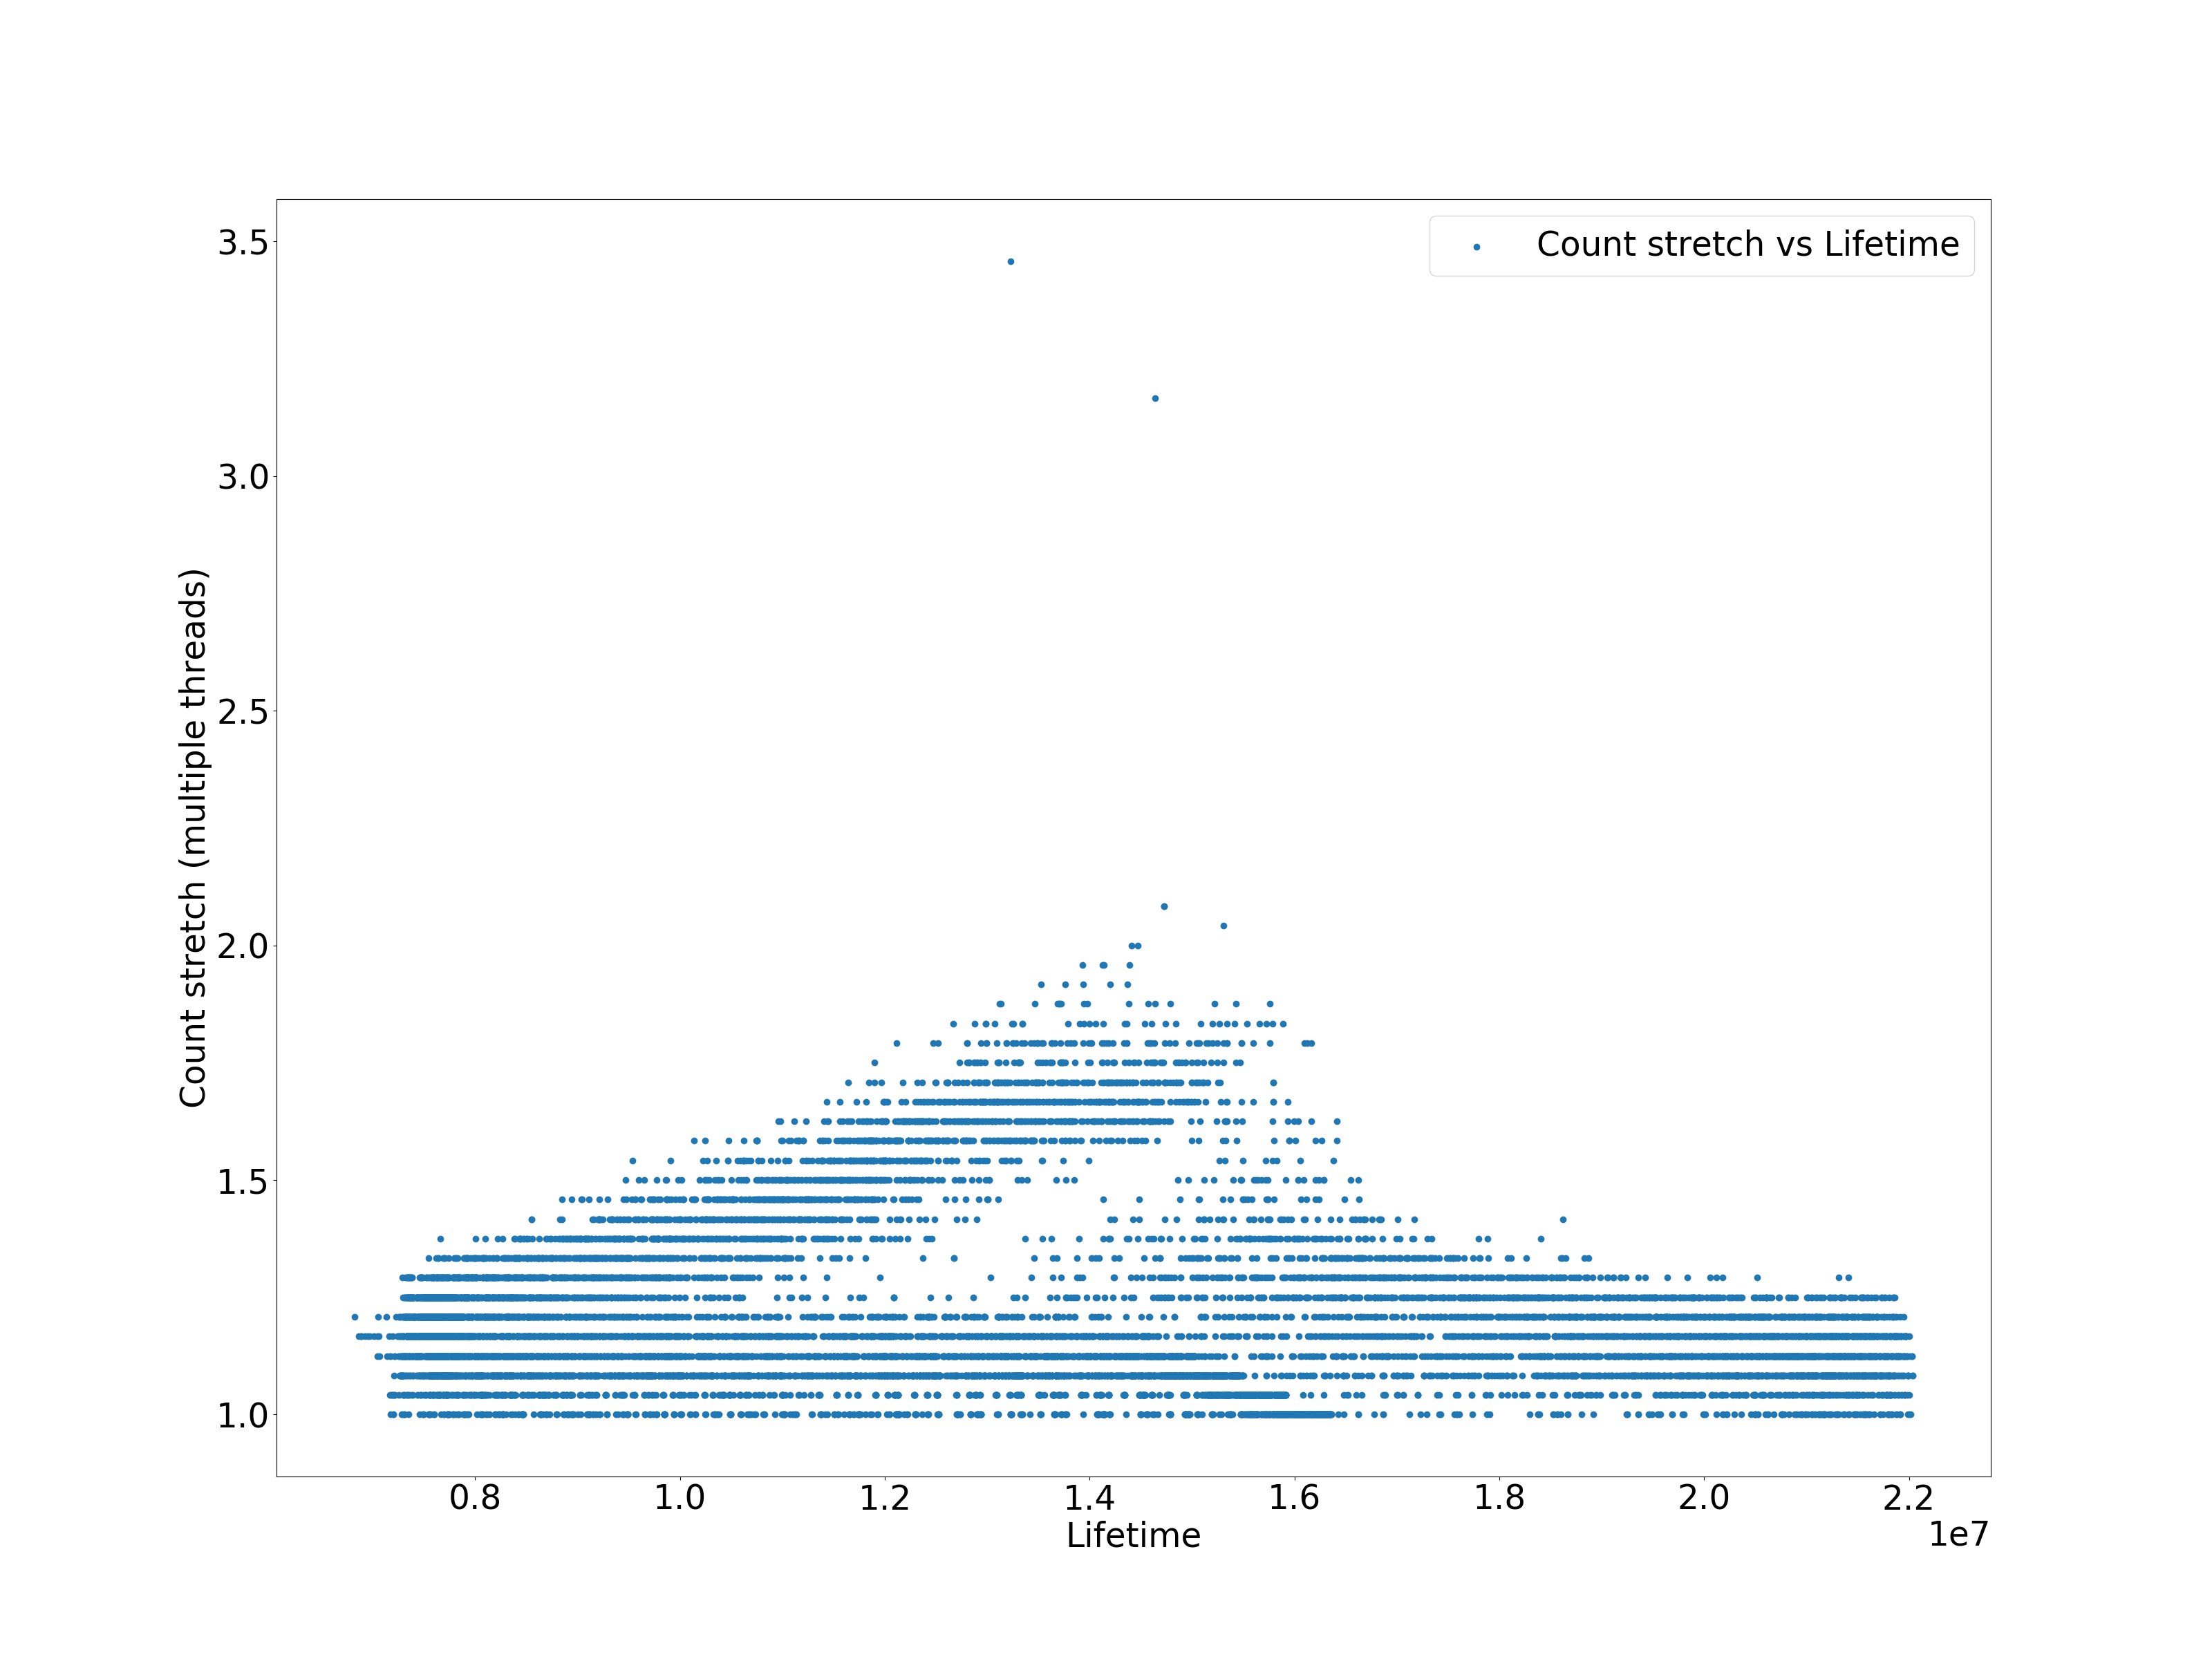
\includegraphics[width=\linewidth]{../LERT-src/sigmod20_figs/countstretch-lifetime.png}
  \captionsetup{margin=.5cm}
  \caption{Distribution of count stretch vs lifetime of reported items in a
    CSL with 8 cones and 8 threads.}
  \label{fig:countstretch-analysis}
\end{subfigure}
\\
\begin{subfigure}{.50\textwidth}
  \centering
  %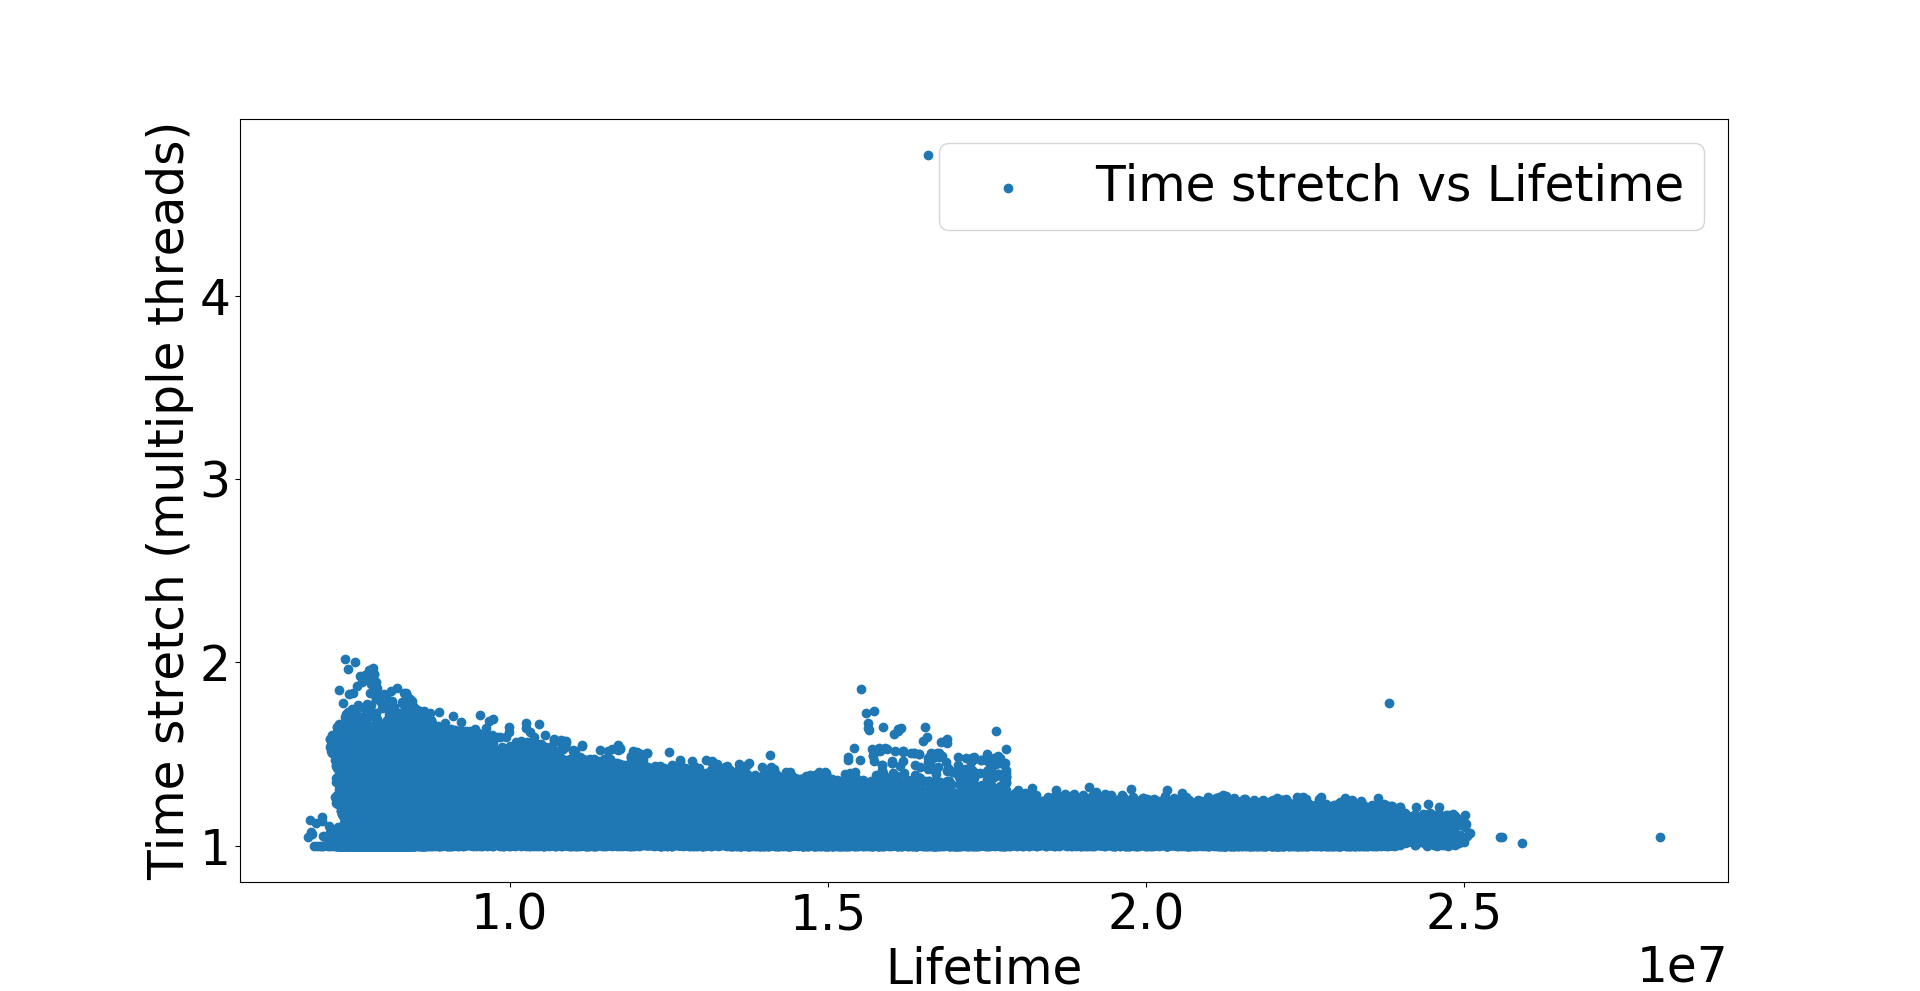
\includegraphics[width=.8\linewidth]{fig/Time-Stretch-Lifetime_r23_l4.png}
  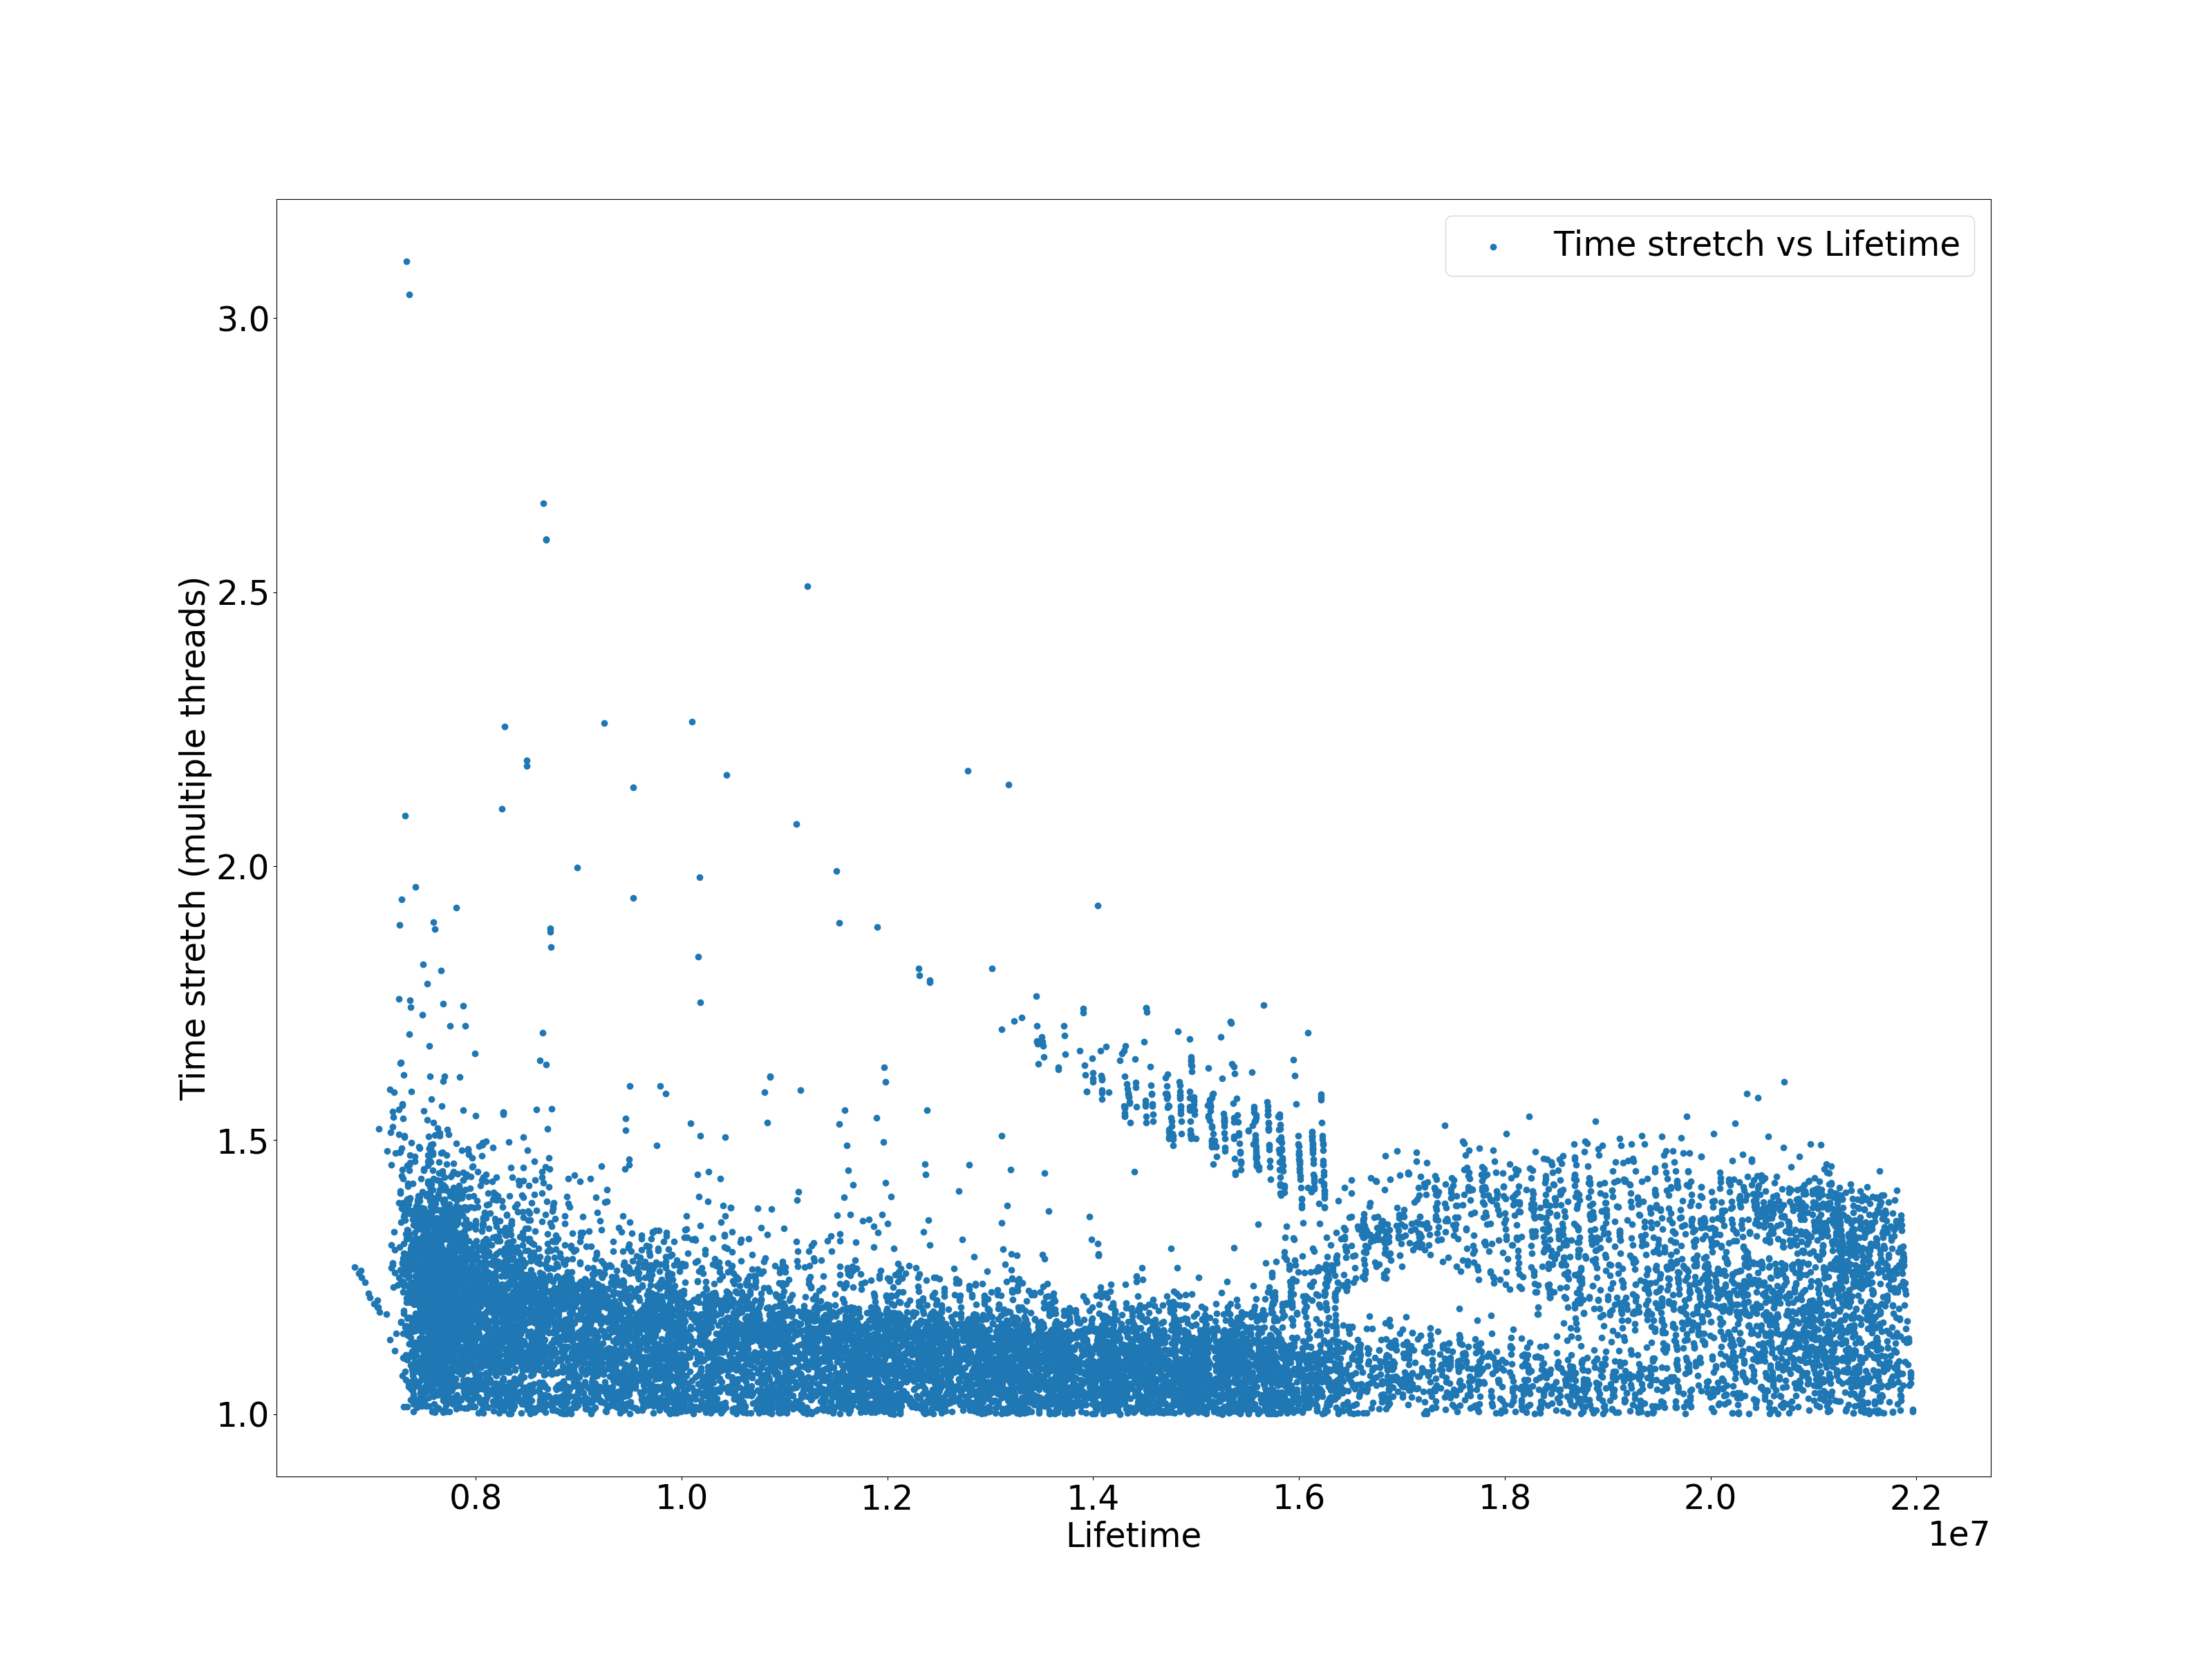
\includegraphics[width=\linewidth]{../LERT-src/sigmod20_figs/timestretch-lifetime.png}
  \captionsetup{margin=.5cm}
  \caption{Distribution of time stretch vs lifetime of reported items in a
    TSL with 8 cones and 8 threads.}
  \label{fig:timestretch-analysis}
\end{subfigure}
}
\caption{Data structure configuration: RAM level: 8388608 slots in
    the CQF, levels: 4, growth factor: 4, level thresholds for on-disk
    level: (2, 4, 8), cones: 8, threads: 8, number of
  observations: 512M.
}
\label{fig:stretch-analysis}
\end{figure}


\subsection{Experimental setup}
\label{setup}

We describe how we designed experiments to answer the questions 
above. We describe our workloads, 
and how we validated timeliness and measured I/O performance.

\ourparagraph{Workload} Firehose~\cite{AndersonPl13} is a suite of benchmarks
simulating a network-event monitoring workload. A Firehose benchmark
consists of a \textit{generator} that feeds keys to the \textit{analytic},
being benchmarked. The analytic must detect
and report each key that has $24$ observations.

Firehose includes two generators: the power-law generator selects from
a static ground set of 100,000 keys according to a power-law distribution, while
the active-set generator allows the ground set to drift over an infinite key
space. We use the active-set generator 
because an infinite key space more closely matches many real world streaming workloads. 
To simulate a stream of keys drawn from a huge key-space we increase the key space
of the active set to one million.


\ourparagraph{Other workloads}\label{diff_dist} Apart from Firehose, we use four other
simulated workloads to evaluate the empirical stretch in the \ts. These four
workloads are generated to show the robustness of
the data structure to non-power-law distributions. In the first
distribution, $M$ (where $M$ is the size of the level in RAM) keys appear with a
count between 24--50 and rest of the keys are chosen uniformly at random from a
big universe. In the second, $M$ keys appear 24 times and the rest of the keys
appear 23 times. In the third, $M$ keys appear round robin each with a
count $>24$. In the fourth, for each key we pick the count uniformly at random
between 1--25.

\ourparagraph{Reporting} During insertion, we record each reported
item and the index in the stream at which it is reported by the data structure.
We record by inserting the reported item in an exact CQF (anomaly CQF) and
encoding the index as the count of the item in the anomaly CQF.
%
We also use the anomaly CQF to check if an incoming item has already been
reported. 
We only insert the item if
it is not reported yet. This prevents duplicate reports. 

\ourparagraph{Timeliness} For the timeliness evaluation, we measure the reporting delay
after its $T$th occurrence. We have two measures
of timeliness: time stretch and count stretch.

The \ts upper bounds the reporting delay  of an item based on its lifetime (i.e. time between its first
and $T$th instance). To validate the
timeliness of the \ts, we first perform an offline analysis of the stream and calculate the
lifetime of each reportable item.
%
Given a reporting threshold $T$, we record the index of the first occurrence of
the item ($I_0$) and the index of the $T$-th occurrence of the item ($I_T$).
%
During ingestion, we record the index ($I_R$) at which the \ts reports the item.
We calculate the time stretch ($ts$) for each
reported item as $ts = (I_R-I_0)/(I_T-I_0)$ and verify that $ts \leq (1+
\alpha)$.

Multiple threads process chunks of 1024
observations from the input stream.  We consider all reports a thread generates 
while processing the $i$th observation to occur
at time $i$.  Due to concurrency, two observations
of the same key may be inserted into the data structure in a
different order than they are pulled off of the input stream.  This
may introduce some noise in our time-stretch measurements.  However,
our experimental results with and without multi-threading were nearly
identical, indicating that the noise is small.

In the \cs, the upper bound is on the count of the item when it is reported. To
validate timeliness, we first record indexes at which items are reported by
the \cs ($I_R$). We then perform an offline analysis to determine the count of
the item at index $I_R$ ($C_{I_R}$) in the stream. We then calculate the count
stretch ($cs$) as $cs=C_{I_R}/T$ and validate that $cs \leq (T+\sum_{i=1}^{L}
\tau_i)/T$.

To perform the offline analysis of the stream we first generate the stream from
the active-set generator and dump it in a file. We then read the stream from the
file for the analysis and for streaming it to the data structure. For timeliness
validation experiments we use a stream of 512 Million observations from the
active-set generator.

\ourparagraph{I/O performance} In our implementation of the time-stretch,
count-stretch and immediate-report \LERT, we allocate space for the data structure by mmap-ing each level (i.e., the CQF)
to a file on SSD. To force the data structure to keep all levels except
the first one on SSD we limit the RAM available to the insertion process using
the ``cgroups'' utility in linux.
%
We calculate the total RAM needed by the insertion process to only keep the
first level in RAM by adding the size of the first level, the space used by the
anomaly CQF to record reported keys, the space used by thread-local buffers, and
a small amount of extra space to read the stream sequentially from SSD. We then
provision the RAM to the next power-of-two of the total sum.

To measure the total I/O performed by the data structure we use the ``iotop''
utility in linux.  Using \texttt{iotop} we can measure the total amount of reads
and writes in KB performed by the process doing insertions.

To validate, we calculate the total amount of I/O performed by the data
structure based on the number of merges (shuffle-merges in case of the \cs) and
\ts and sizes of levels involved in those merges.

Similar to validation experiments, we first dump the stream to a file and then
feed the stream to the data structure by streaming it from the file. We use a
stream of 64 Million observations from the active-set generator.

\ourparagraph{Average insertion throughput and scalability}
To measure the average insertion throughput, we first
generate the stream from the active-set generator and dump it in a file. We then
feed the stream to the data structure by streaming it from the file and measure
the total time.

To evaluate scalability, we measure how data-structure throughput
changes with increasing number of threads. We
evaluate power-of-2 thread counts between $1$ and $64$.

To deamortize the data structures we divide them into $2048$ cones. We use a
stream of $4$ Billion observations from the active-set generator.
We evaluate the
insertion performance and scalability for three values (16, 32 and 64) of the
DatasetSize-to-RAM-ratio (i.e., the ratio of the data set size to the available RAM).

\ourparagraph{Instantaneous insertion throughput} We also evaluate the
instantaneous throughput of the data structure when run using either a single cone and
thread or  multiple cones and threads. We approximate instantaneous throughput by
calculating throughput (using system timestamps) every $\kappa$ observations.
In our evaluation, we fix $\kappa = 2^{17}$.

\ourparagraph{Machine specifications} The OS for all experiments 
was $64$-bit Ubuntu 18.04 running Linux kernel 4.15.0-34-generic
%
The machine for all timeliness and I/O performance benchmarks 
had an Intel Skylake CPU (Core(TM) i7-6700HQ CPU @ $2.60$GHz with $4$ cores
and $6$MB L$3$ cache) with $32$ GB RAM and a $1$TB Toshiba SSD.
%
The machine for all scalability benchmarks had an Intel
Xeon(R) CPU (E5-2683 v4 @ 2.10GHz with $64$ cores and $20$MB L$3$ cache) with
$512$ GB RAM and a $1$TB Samsung $860$ SSD.

For all the experiments, we use a reporting threshold of $24$ since it is the default in the Firehose benchmarking suite.

\begin{figure}
{\centering
\begin{subfigure}{.50\textwidth}
  \centering
  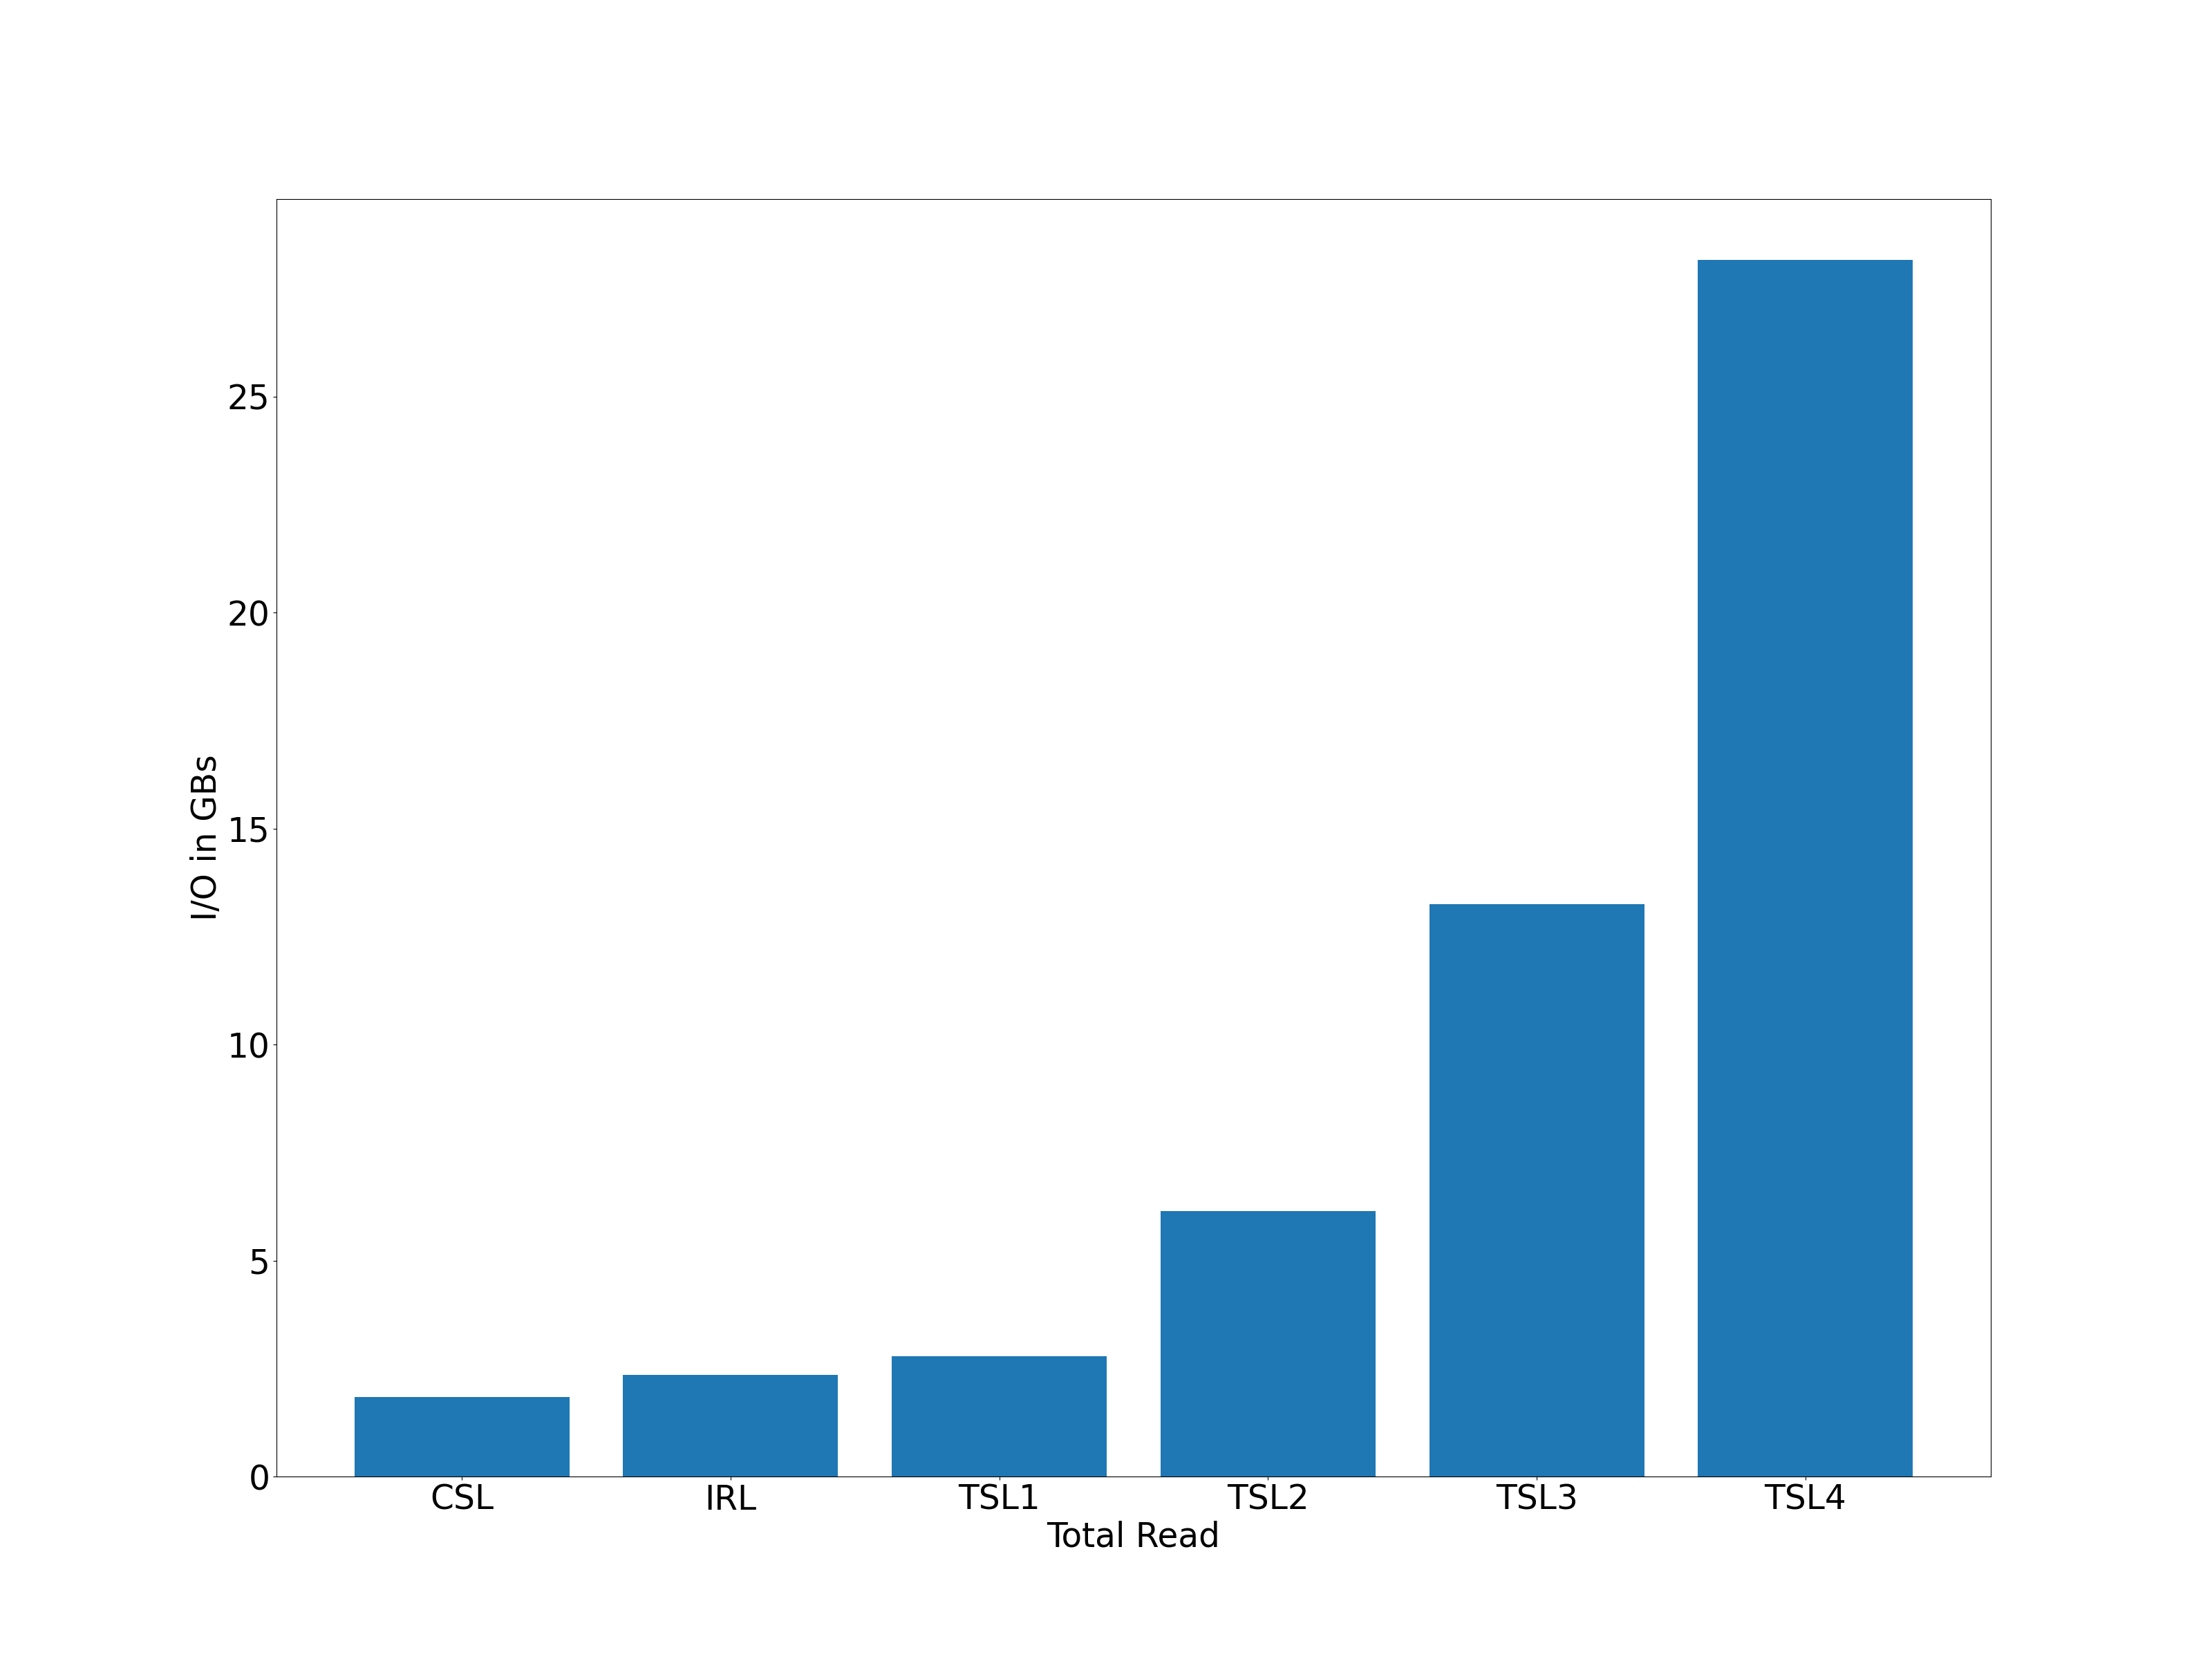
\includegraphics[width=\linewidth]{../LERT-src/sigmod20_figs/io_read.png}
  \captionsetup{margin=.5cm}
 \caption{Reads I/O}
\end{subfigure}
\\
\begin{subfigure}{.50\textwidth}
  \centering
  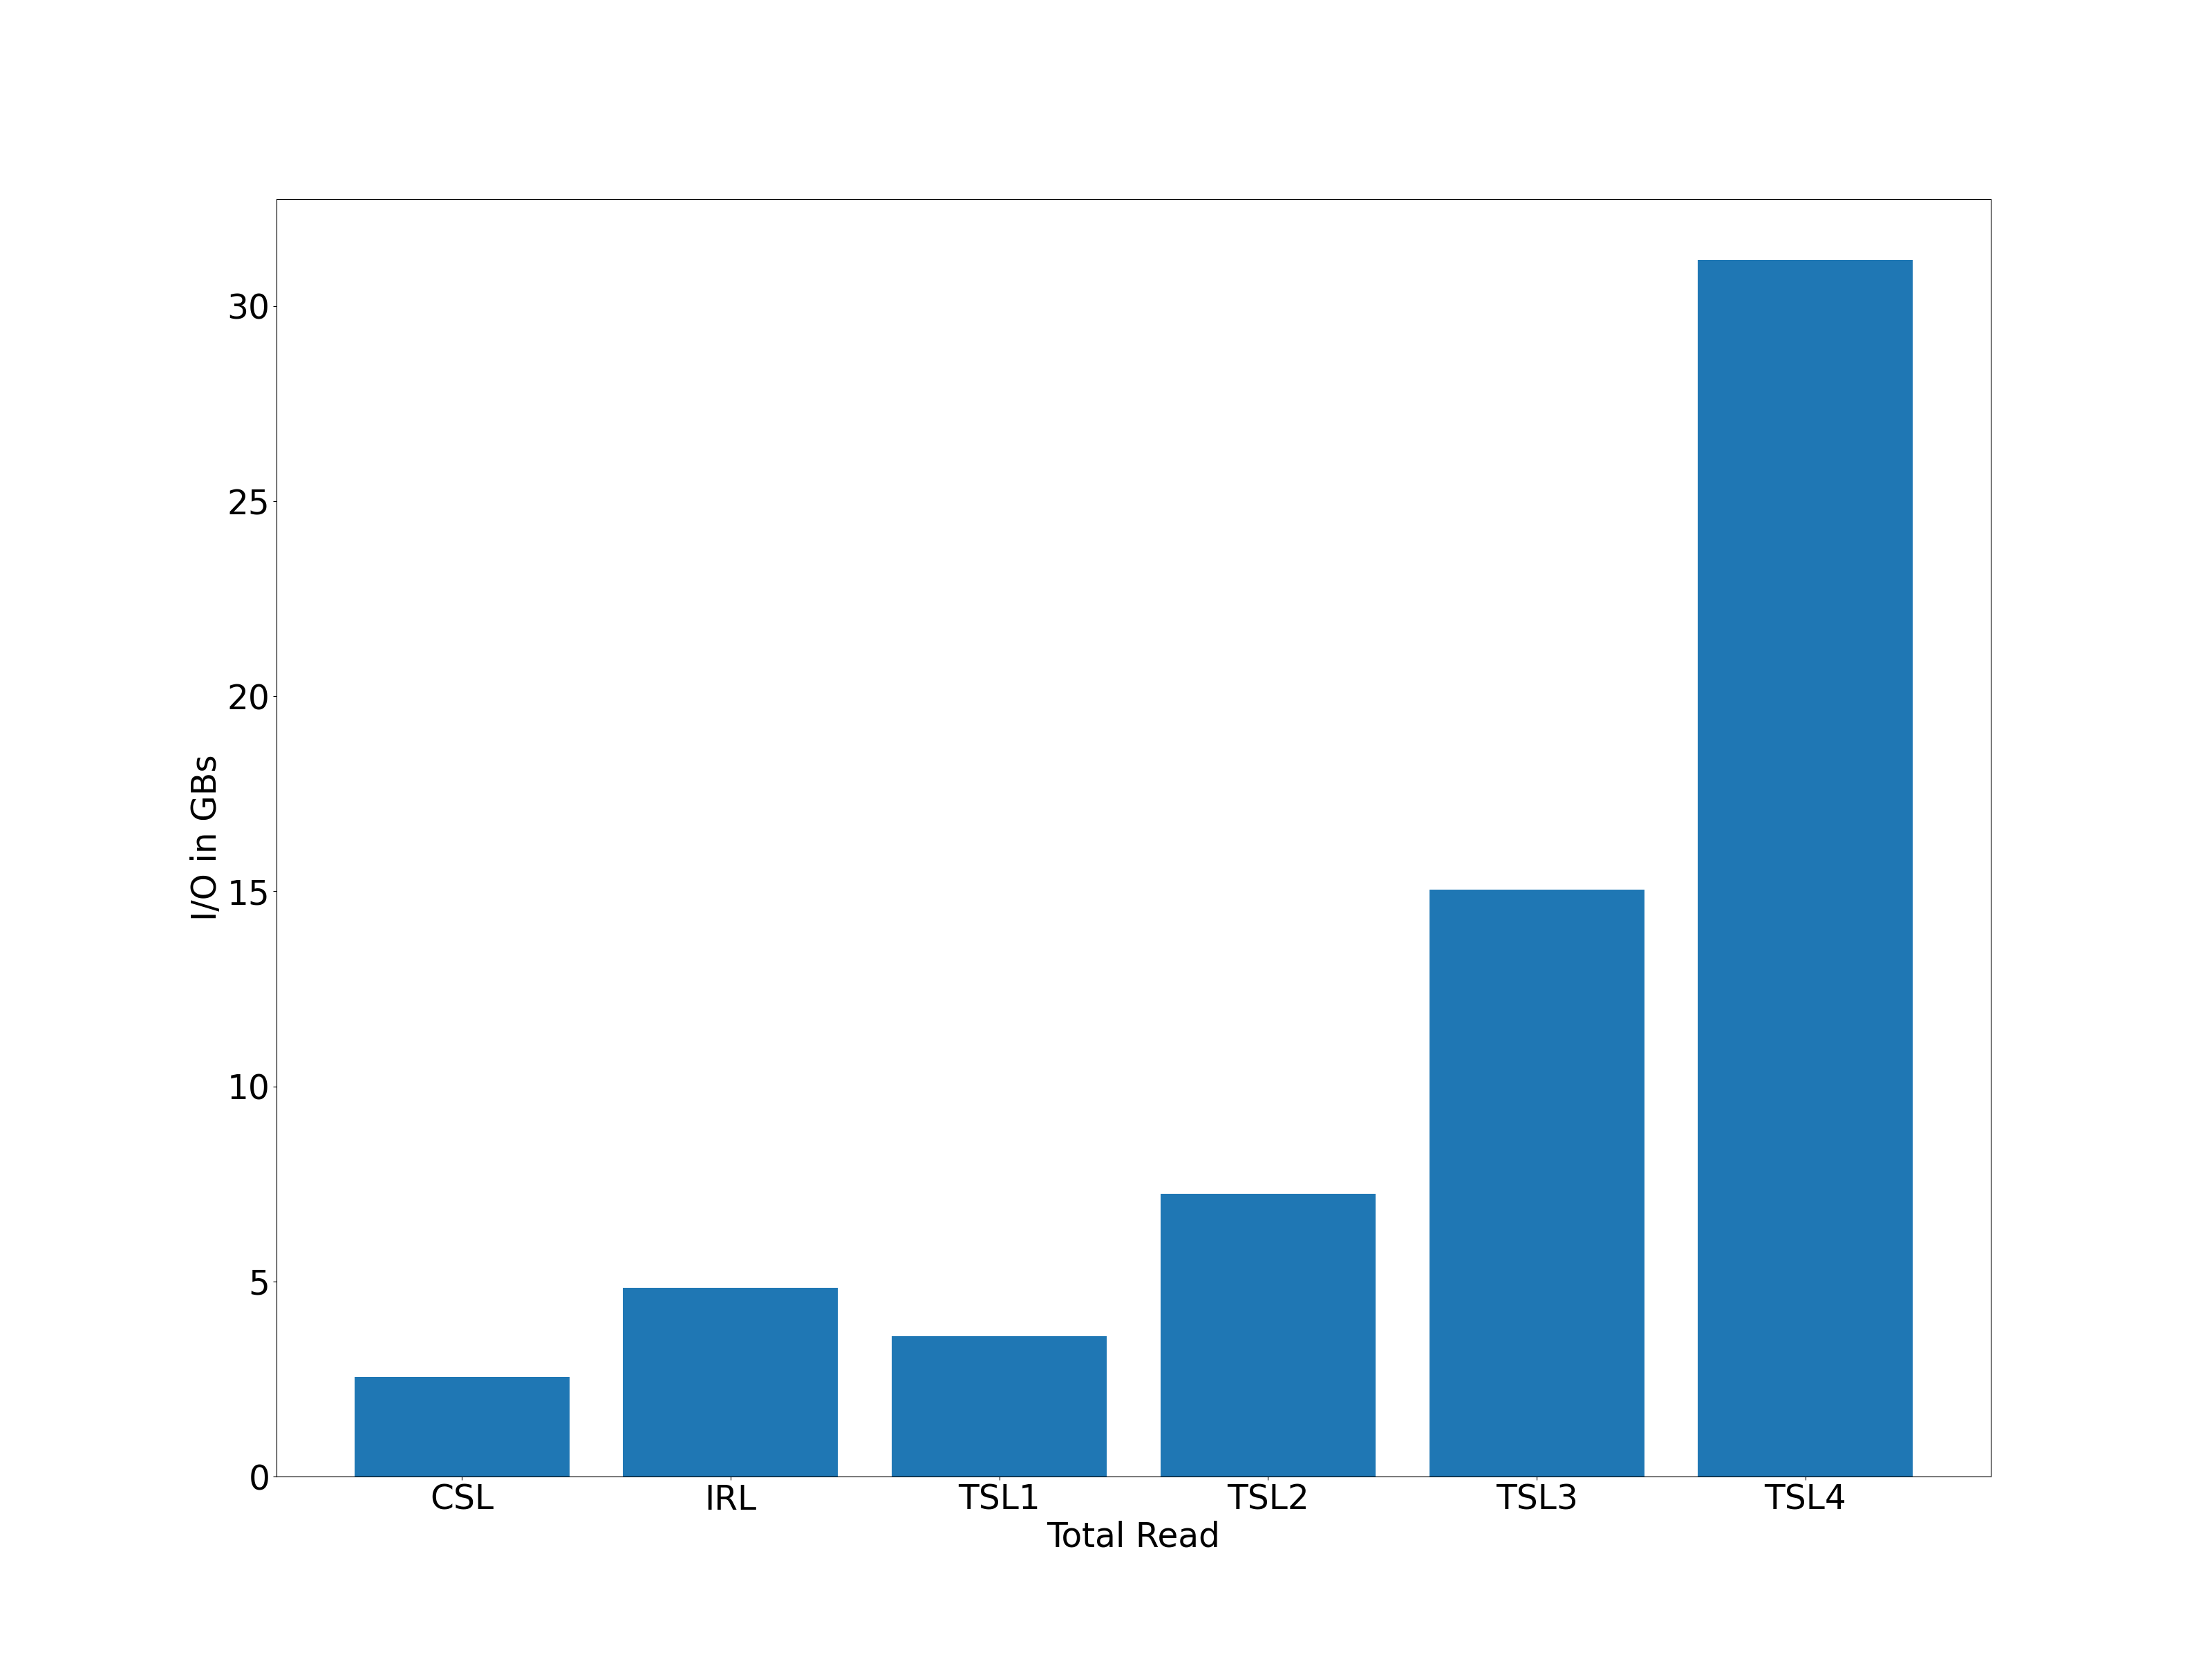
\includegraphics[width=\linewidth]{../LERT-src/sigmod20_figs/io_write.png}
  \captionsetup{margin=.5cm}
 \caption{Write I/O}
\end{subfigure}
}
\label{fig:io-data}
\caption{Total
  I/O performed by the count-stretch, time-stretch and immediate report \LERT. Data structure configuration: RAM
  level: 4194304 slots in the CQF, levels: 3, growth factor: 4, number of
  observations: 64M. Immediate-report LERT (IRL).}
\end{figure}

%\begin{figure}
  %\begin{centering}
    %\begin{tikzpicture}[]
    %\begin{groupplot} [
      %group style = {group name=my plots, group size = 1 by 2,},
      %ybar,
      %ymajorgrids,
      %legend style={at={(0.8,2.2)}},
      %symbolic x coords={CSL, IRL, TSL1, TSL2, TSL3, TSL4},
      %ymin=0,
      %%xlabel={Data structures},
      %nodes near coords align={vertical},
      %legend columns=2,
      %%width=.4\textwidth,
      %width=8cm, height=4cm,
      %%scale=0.7,
      %%enlarge x limits=false,enlarge y limits=false,
      %]
      %\nextgroupplot[ylabel={I/O in GBs}]
        %\addplot[pattern=crosshatch, pattern color=teal]  coordinates{
          %(CSL, 1.398141) (IRL, 1.453542) (TSL1, 2.311195)
          %(TSL2, 5.070866) (TSL3, 10.797431) (TSL4, 22.592907)
      %};
        %\addplot[pattern=grid, pattern color=red]        coordinates {
          %(CSL, 1.157115) (IRL, 1.782303) (TSL1, 2.034367)
          %(TSL2, 4.680427) (TSL3, 10.207707) (TSL4, 21.591663)
        %};
        %\nextgroupplot[ylabel={I/O in GBs}, xlabel={Data structures}]
        %\addplot[pattern=crosshatch, pattern color=teal] coordinates{
          %(CSL, 1.615197) (IRL, 1.678316) (TSL1, 2.655848)
          %(TSL2, 5.799339) (TSL3, 12.318755) (TSL4, 25.733310)
        %};
        %\addplot[pattern=grid, pattern color=red]   coordinates {
          %(CSL, 1.811719) (IRL, 1.684229) (TSL1, 2.698935)
          %(TSL2, 5.390067) (TSL3, 11.194569) (TSL4, 23.095296)
        %};
        %\legend{Calculated, Measured}
  %\end{groupplot}
  %\node[text width=2cm,align=center,anchor=north] at ([yshift=-2mm]my plots c1r1.south)
  %{\subcaption{Reads \label{subplot:read-io}}};
  %\node[text width=2cm,align=center,anchor=north] at ([yshift=-8mm]my plots c1r2.south)
  %{\subcaption{Writes \label{subplot:write-io}}};
  %\end{tikzpicture}
%\end{centering}
%\caption{Total
  %I/O performed by the count-stretch, time-stretch and immediate report \LERT. Data structure configuration: RAM
  %level: 4194304 slots in the CQF, levels: 3, growth factor: 4, number of
  %observations: 64M. Immediate-report LERT (IRL).}
    %\label{fig:io-data}
%\end{figure}

\begin{figure*}
\centering
{
 %\begin{subfigure}{0.32\linewidth}
%\centering
%\begin{tikzpicture}[yscale=.6, xscale=.7]
 %\begin{axis}[
    %ybar,
    %ymajorgrids,
    %xlabel={Data structures},
    %nodes near coords align={vertical},
    %legend style={at={(0.5,1)},
        %anchor=north,legend columns=-1},
    %symbolic x coords={MG, CSL, IRL, TSL1, TSL2, TSL3, TSL4},
    %ymin=0,
    %bar width=20pt,
    %xtick=data,
    %ylabel={Insertion throughput (Million ops/sec)},
  %]
  %\addplot[fill=teal] coordinates{
  %(MG, 2.2) (CSL, .93808630) (IRL, .46935135) (TSL1, .48538976)
  %(TSL2, .24639038) (TSL3, .12283503) (TSL4, .06085242)};
 %\end{axis}
%\end{tikzpicture}
 %\caption{Items inserted per second by the CSL, TSL, IRL and
 %Misra-Gries (MG) data structure. MG is in-memory.}
 %\label{fig:throughput-data}
%\end{subfigure}
%
\begin{subfigure}{0.33\linewidth}
  \centering
  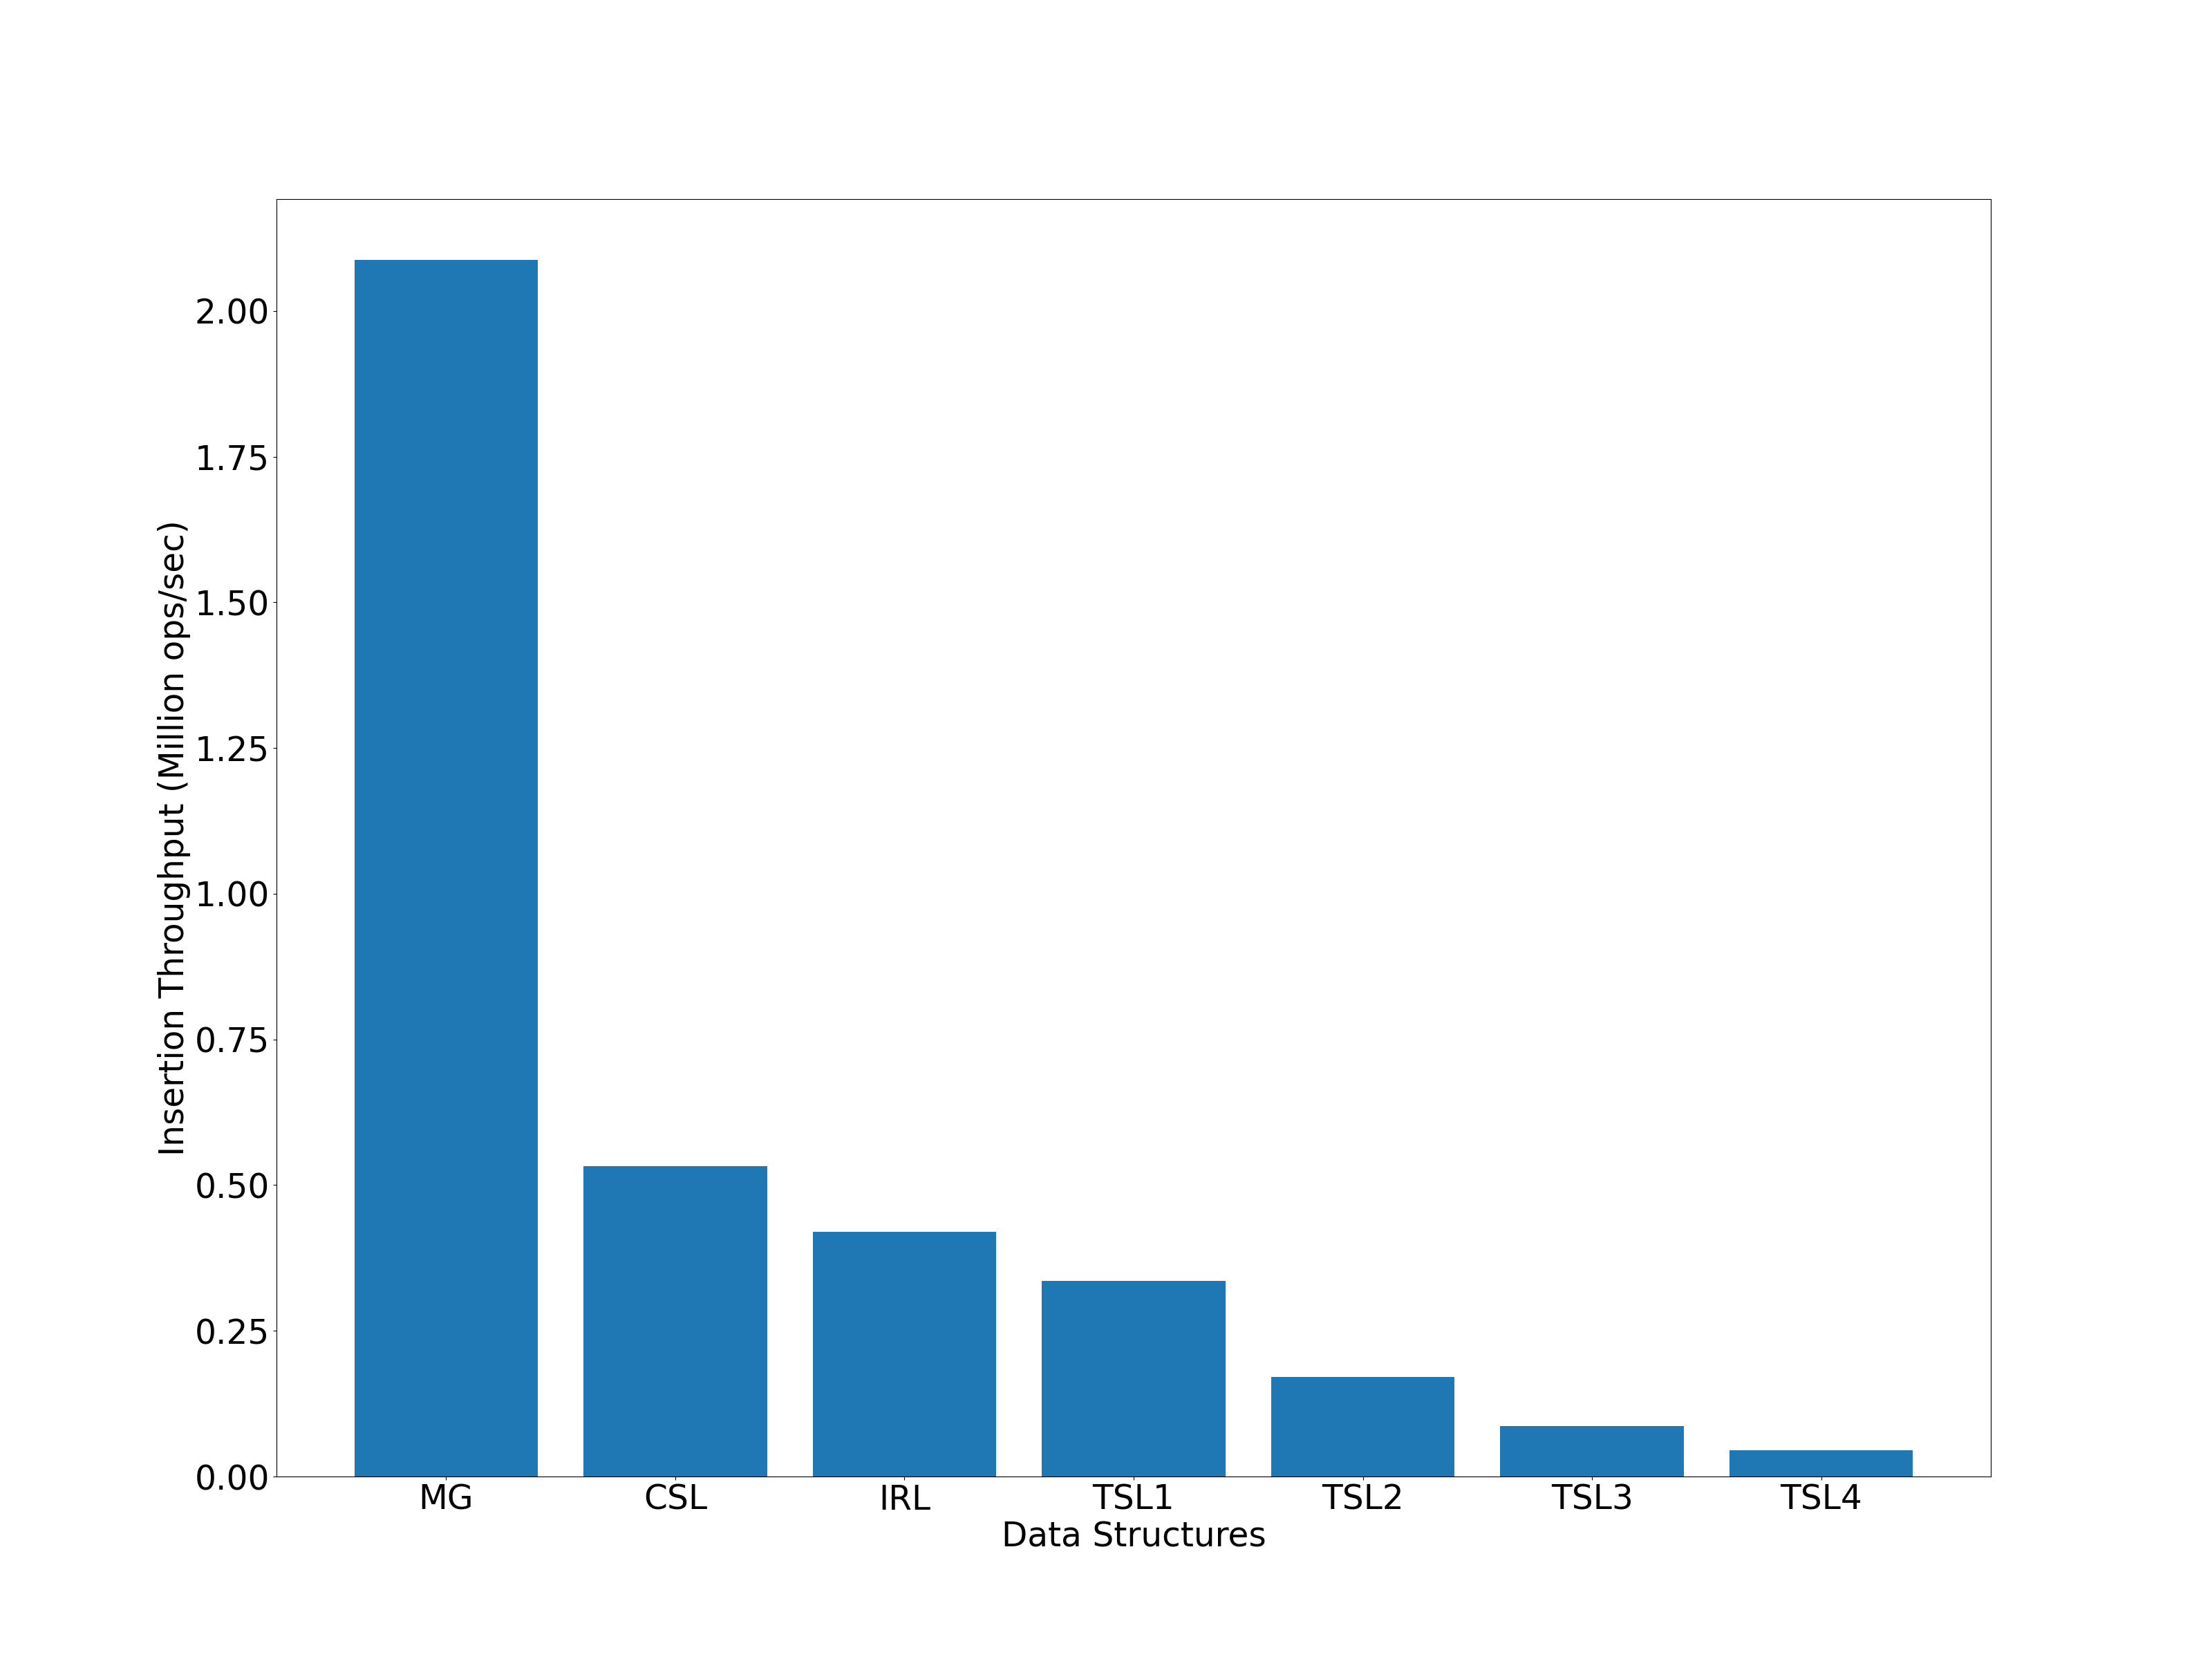
\includegraphics[width=\linewidth]{../LERT-src/sigmod20_figs/throughput.png}
  %\captionsetup{margin=.5cm}
 \caption{Items inserted per second by the CSL, TSL, IRL and
 Misra-Gries (MG) data structure. MG is in-memory.}
 \label{fig:throughput-data}
\end{subfigure}
\hfill
%
\hfill
\begin{subfigure}{0.32\linewidth}
  \centering
  \captionsetup[subfigure]{justification=centering}
  {\centering
      \begin{tikzpicture}[yscale=0.7, xscale=0.8]
        \begin{axis}[
            width=\linewidth,
            scale only axis,
            xlabel={Number of threads},
            ylabel={Throughput (Million inserts/sec)},
            xmin=0,
            ymin=0,
            xmax=75,
            %ymin=0,
            %ymax=55,
            %xtick={1,2,3,4},
            grid=major,
            legend entries={Ratio: 16, Ratio: 32, Ratio: 64},
            %legend entries={Ratio: 16, Ratio: 32, MG in-memory},
            legend style={legend pos=south east},
            scaled y ticks=false,
          ]
          \addplot[color=blue,mark=pentagon*]       table
          {data/popcornfilter-threads-4B-c2048-q15-l4-r2G.txt};
          %{../LERT-src/sigmod20_raw/scalability_throughput_16.output};
          \addplot[color=teal,mark=square*]       table
          {data/popcornfilter-threads-4B-c2048-q15-l4-r1G.txt};
          %{../LERT-src/sigmod20_raw/scalability_throughput_32.output};
          \addplot[color=red,mark=triangle*]       table
          {data/popcornfilter-threads-4B-c2048-q15-l4-r512M.txt};
          %{../LERT-src/sigmod20_raw/scalability_throughput_64.output};
          %\addplot[thick, color=black] coordinates{(0,7.27)(75,7.27)};
        \end{axis}
      \end{tikzpicture}
  }
  \caption{Insertion throughput with increasing number of threads for the
    \cs on 4 Billion observations. }
    \label{fig:time-threads-pf}
\end{subfigure}
%
\hfill
\begin{subfigure}{0.33\linewidth}
  \centering
  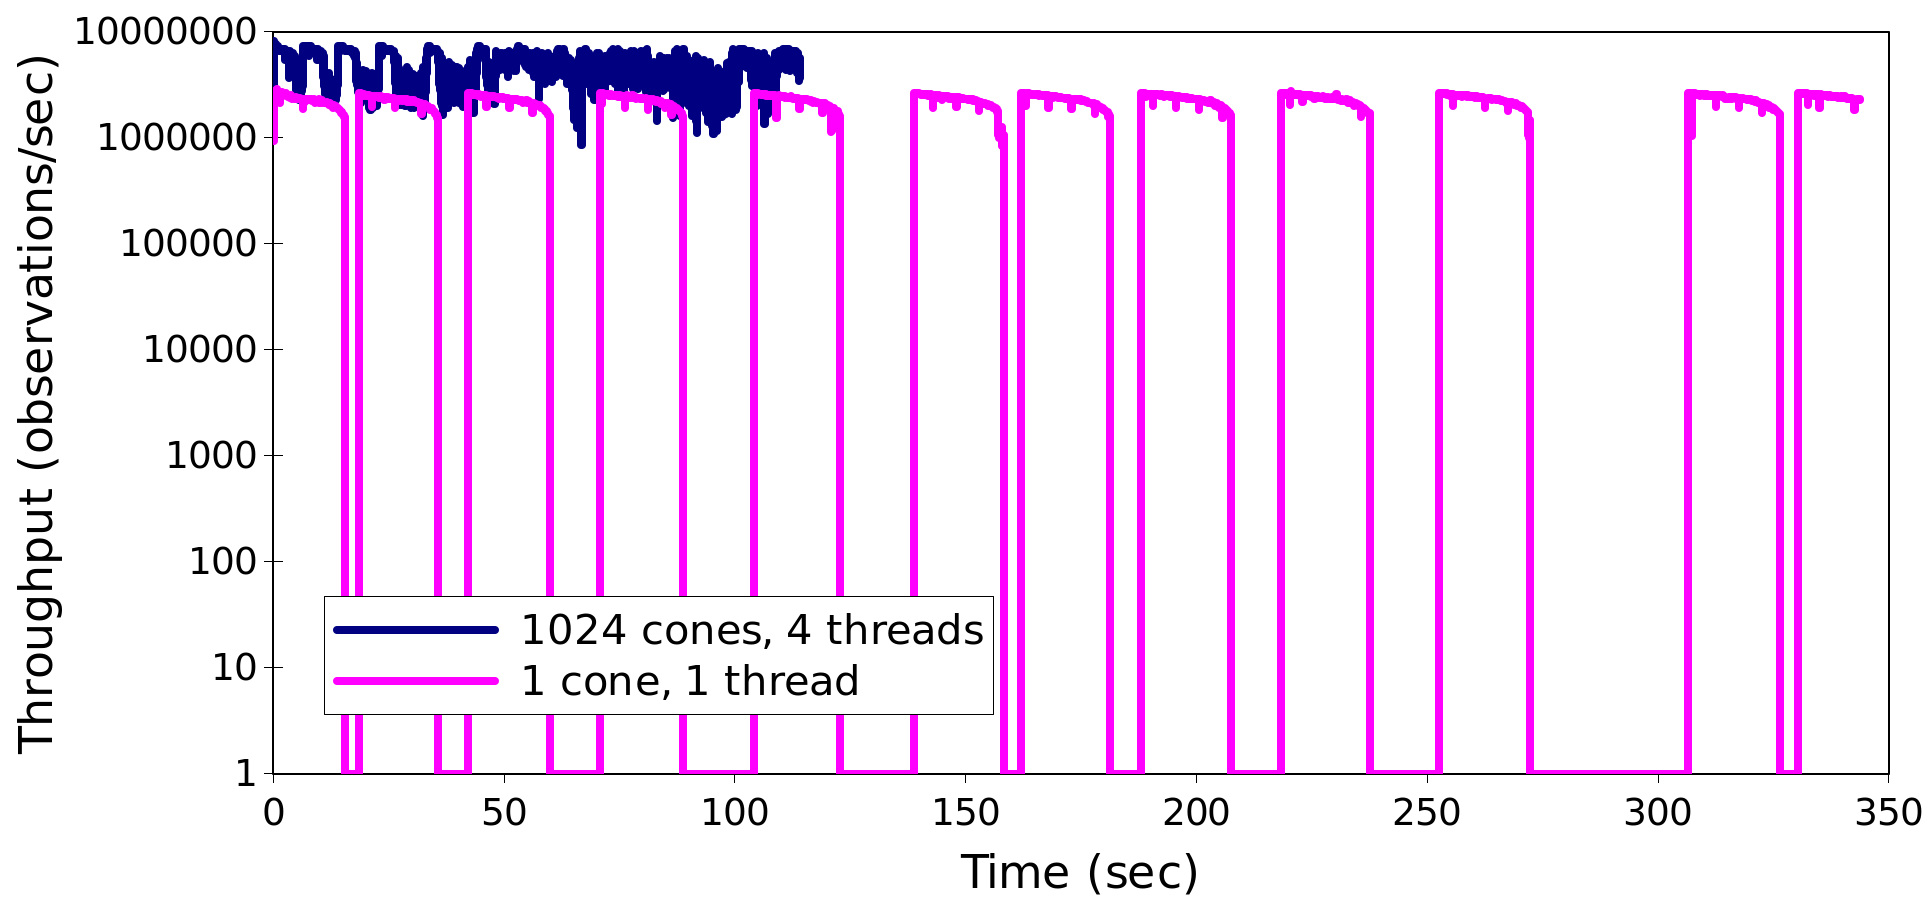
\includegraphics[width=\linewidth]{fig/ThroughputAnalysis.png}
  %\captionsetup{margin=.5cm}
  \caption{Instantaneous throughput of the \cs with 1 cone and 1 thread and 1024
  cones and 4 threads.}
  \label{fig:throughputanalysis}
\end{subfigure}
}
\caption{Data structure configuration for (a): RAM level: 4194304 slots in
    the CQF, levels: 3, growth factor: 4, number of observations: 64M.
    DatasetSize-to-RAM-ratio: 12.5. For (b):
    RAM level: 67108864 slots in the CQF, levels: 4, growth factor: 4, level
    thresholds for on-disk level($\ell_3\ldots\ell_{1}$): (2, 4, 8), cones: 2048
    with greedy flushing, DatasetSize-to-RAM-ratio: 16, 32, and 64. For (c):
    Same as ~\Cref{fig:countstretch}.}
\end{figure*}




\subsection{Timely reporting}
\label{timely-reporting}

\ourparagraph{Cascade filter} \Cref{fig:countstretch,fig:timestretch} 
show the distribution of count stretch and time stretch of reported items in the
cascade filter. The cascade filter's maximum count-stretch is $3.0$ and maximum time stretch is $>12$,
much higher than 
any single-threaded 
count-stretch or \ts.

\ourparagraph{\Cs} \Cref{fig:countstretch} validates worst-case count stretch
for the \cs.
The total on-disk count for an element
is 14, so the maximum possible count when reported is $38$ (i.e.,
$24+14$), for a maximum count stretch of $1.583$.  The maximum reported count
stretch is $1.583$.
%

\ourparagraph{\Ts} ~\Cref{fig:timestretch} shows the \ts meets the time-stretch requirements.
%
The maximum reported time stretch is $1.59$ which is smaller than the maximum
allowable time stretch of $2$.
%
~\Cref{fig:timeliness-timestretch} shows the distribution of empirical time
stretches with changing $\alpha$ values. The time stretch of any
reported element is always smaller than the maximum allowable time stretch.  As
the number of age bits increases, $\alpha$ decreases and the time stretch decreases.

\subsection{Robustness with input distributions}

\Cref{fig:timestretch-arb} shows the robustness of empirical time stretch (ETS) on
four input distributions other than the Firehose power-law distribution.
The ETS is less than 2, the theoretical
limit of the data structure for all input distributions.

\subsection{Effect of deamortization/threading}
\label{multi-delay}

\Cref{fig:countstretch,fig:timestretch} show the effect of
deamortization and multi-threading on timeliness in the \cs and \ts.

Using $8$ cones instead of one does not change the timeliness of any reported
item.
%
This is because the distribution of items in the stream is random (see
\Cref{setup}) and we use a uniform-random hash function to distribute items to
each cone. Each cone gets a similar number of items and the cones perform
shuffle-merges in sync (refer to~\Cref{timeliness-cone-theory}).

Running the count-stretch and time-stretch \LERT with $8$ cones and $8$ threads
does affect timeliness of reported items. Some items are reported later than the
theoretical upper bound. The reported maximum time- and count-stretch is
$>5$.
%
This is because each thread inserts items into a local buffer when it can not
immediately acquire the cone lock.  We empty local buffers only when they are
full.
%
The maximum delay happens when an item's lifetime is similar to the time it
takes for a cone to incur a full flush involving all levels of the data
structure.~\Cref{fig:stretch-analysis} shows the stretch of reported items and
their lifetime. The maximum-stretch items have a
lifetime $\approx16$M observations which is the number of observations it takes
for a cone to incur a full flush.

\subsection{Effect of buffering}
\Cref{fig:countstretch-buffering} shows the empirical count stretch with three
different buffering strategies. In the first, we use buffers without
any constraint on the count of a key inside a buffer. We dump the buffer into
the main data structure when it is full. In the second, we constrain the maximum
count a key can have in a buffer to~$T/P$ (for $T=24$ and $P=8$ the max count
is 3). In the third, we don't use buffers. Threads try to acquire the lock on
the cone and wait if the lock is not available.

The empirical stretch is smallest without  buffers.
However, not using the buffers increases contention among
threads and reduces insertion throughput. Using the buffers is
$2.5\times$ faster compared to not using the buffer.

\subsection{I/O performance and throughput}

\Cref{fig:io-data} shows the total amount of I/O 
performed by the count-stretch, time-stretch and immediate-report \LERT while ingesting a stream. For all data
structures, the total I/O calculated and total I/O measured using \texttt{iotop}
is similar.

The \cs does the least I/O because it performs the fewest
shuffle-merges. The I/O for the \ts grows by a factor of two as 
the number of bins increases, as predicted by the theory. The I/O for \ps
is similar to that of the \ts with stretch 2.
This shows that
when item counts follow a power-law distribution, we can achieve immediate
reporting with the same amount of I/O as with a time stretch of 2.

\ourparagraph{Insertion throughput}
\Cref{fig:throughput-data} shows
insertion throughput using the same configuration and stream
as the total-I/O experiments.
%
The \cs has the highest throughput
because it performs the fewest I/Os. The \ps
has lower throughput because it performs extra random point queries. The \ts throughput decreases as we add bins and decrease
the stretch.

The {\bf Misra-Gries data structure}
throughput is $2.2$ Million ops/sec in-memory. This acts a baseline for
in-memory insertion throughput. The in-memory MG data structure is only twice as
fast as the on-disk \cs.

\subsection{Instantaneous throughput} 

\Cref{fig:throughputanalysis} shows the instantaneous throughput of the
\cs. De-amortization and multi-threading improve both average throughput and
throughput variance.  With one thread and one cone, the data structure
periodically stops processing inputs to perform flushes, causing throughput to
crash to 0.  With 1024 cones and four threads, the system has much smoother
throughput, never stops processing inputs, and has about 3$\times$ greater
average throughput.


\subsection{Scaling with multiple threads}\label{scalability}

\Cref{fig:time-threads-pf} shows \cs throughput with increasing
number of threads. 
The 
scalability will follow
for other variants 
since they all have the same insertion and SSD
access pattern.
%
The insertion throughput increases with thread count. 
We used three values of DatasetSize-to-RAM-ratio: 16, 32, and 64.
All have similar scalability curves.


\end{document}

